% This must be in the first 5 lines to tell arXiv to use pdfLaTeX, which is strongly recommended.
\pdfoutput=1
% In particular, the hyperref package requires pdfLaTeX in order to break URLs across lines.

\documentclass[11pt]{article}

% Remove the "review" option to generate the final version.
\usepackage{acl}

% Standard package includes
\usepackage{times}
\usepackage{latexsym}

% For proper rendering and hyphenation of words containing Latin characters (including in bib files)
\usepackage[T1]{fontenc}
% For Vietnamese characters
% \usepackage[T5]{fontenc}
% See https://www.latex-project.org/help/documentation/encguide.pdf for other character sets

% This assumes your files are encoded as UTF8
\usepackage[utf8]{inputenc}

% This is not strictly necessary, and may be commented out,
% but it will improve the layout of the manuscript,
% and will typically save some space.
\usepackage{microtype}

% If the title and author information does not fit in the area allocated, uncomment the following
%
%\setlength\titlebox{<dim>}
%
% and set <dim> to something 5cm or larger.

\usepackage{tcolorbox}
\usepackage{arydshln}
\usepackage{algorithm}
\usepackage{algpseudocode}
\usepackage{ulem}
\usepackage{soul}
\usepackage{xcolor}
\usepackage{todonotes}
\definecolor{mybluei}{RGB}{0,173,239}

\renewcommand{\algorithmicensure}{\textbf{Output:~}}

\usepackage{xspace}
\newcommand{\method}{\mbox{\textsc{TRACER}}\xspace}

\algnewcommand{\LeftComment}[1]{\Statex \(\triangleright\) #1}

\makeatletter
\def\els@aparagraph[#1]#2{\elsparagraph[#1]{#2}}
\def\els@bparagraph#1{\elsparagraph*{#1}}
\makeatother

\title{Wizard of Shopping: Target-Oriented E-commerce Dialogue Generation with Decision Tree Branching}

% Author information can be set in various styles:
% For several authors from the same institution:
% \author{Author 1 \and ... \and Author n \\
%         Address line \\ ... \\ Address line}
% if the names do not fit well on one line use
%         Author 1 \\ {\bf Author 2} \\ ... \\ {\bf Author n} \\
% For authors from different institutions:
% \author{Author 1 \\ Address line \\  ... \\ Address line
%         \And  ... \And
%         Author n \\ Address line \\ ... \\ Address line}
% To start a seperate ``row'' of authors use \AND, as in
% \author{Author 1 \\ Address line \\  ... \\ Address line
%         \AND
%         Author 2 \\ Address line \\ ... \\ Address line \And
%         Author 3 \\ Address line \\ ... \\ Address line}

% \author{First Author \\
%   Affiliation / Address line 1 \\
%   Affiliation / Address line 2 \\
%   Affiliation / Address line 3 \\
%   \texttt{email@domain} \\\And
%   Second Author \\
%   Affiliation / Address line 1 \\
%   Affiliation / Address line 2 \\
%   Affiliation / Address line 3 \\
%   \texttt{email@domain} \\}

\author{Xiangci Li\textsuperscript{\rm 1}$^*$ ~~ Zhiyu Chen\textsuperscript{\rm 2} ~~ Jason Ingyu Choi\textsuperscript{\rm 2}
\AND Nikhita Vedula\textsuperscript{\rm 2} ~~ Besnik Fetahu\textsuperscript{\rm 2} ~~ Oleg Rokhlenko\textsuperscript{\rm 2} ~~ Shervin Malmasi\textsuperscript{\rm 2} \\
  \textsuperscript{\rm 1} AWS AI Labs 
  \textsuperscript{\rm 2} Amazon.com, Inc. \\
  \tt lixiangci8@gmail.com \\ \tt \{zhiyuche, chojson, veduln, besnikf, olegro, malmasi\}@amazon.com \\
}

\begin{document}
\maketitle

\def\thefootnote{*}\footnotetext{~Work performed by the author as a PhD candidate at The University of Texas at Dallas before joining AWS AI Labs.}
\def\thefootnote{\arabic{footnote}}

\begin{abstract}
The goal of conversational product search (CPS) is to develop an intelligent, chat-based shopping assistant that can directly interact with customers to understand shopping intents, ask clarification questions, and find relevant products. However, training such assistants is hindered mainly due to the lack of reliable and large-scale datasets. %Prior studies of CPS are often limited to a very restricted domain (e.g., movie recommendation), or rely on synthetic templates. One alternative is to crowd source high-quality conversations, but this is a nontrivial task given the data noise and steep costs involved.
% interact with a chat-based shopping agent to obtain product recommendations by narrowing down product requirements through dialogue based search. %Prior work on CPS has significant shortcomings. 
%Despite great potential, the development of CPS agents has been challenging. 
Prior human-annotated CPS datasets are extremely small in size and lack integration with real-world product search systems. %Prior studies on CPS focused on representation learning, where the conversations are primarily template-based, lack a natural flow, and are often restricted to fixed domains. %It is also unclear how to extend existing data generation models to a new product domain since these models are usually trained with a fixed dataset. 
We propose a novel approach, \method, which leverages large language models (LLMs) to generate realistic and natural conversations for different shopping domains. \method's novelty lies in grounding the generation to dialogue plans, which are product search trajectories predicted from a decision tree model, that guarantees relevant product discovery in the shortest number of search conditions. 
% collect the first ever large-scale, human-like, target-oriented CPS dataset, called \textit{Wizard-of-Shopping (WoS)}.
% There are three major challenges involved: (1) %Since LLMs are not directly trained with a product catalog, they do not have direct access to product metadata. 
% (1) LLMs are not directly trained with product catalogs and product metadata;
% (2) %LLMs struggle with how and when to ask effective clarification questions to assist customers in quickly discovering their desired products.
% LLMs do not understand when and how to ask clarification questions during search; and (3) %it is unclear how to model customer preferences without real-world shopping data. 
% LLMs can't personalize product searches based on different real-world user preferences. 
% To tackle these, we create dialogue plans that ground LLMs to generate product search conversations, by leveraging decision tree models to select product attributes that uncover the target products.
%we propose a novel \textbf{T}arget-oriented e-comme\textbf{R}ce di\textbf{A}logue generation approach with de\textbf{C}ision tr\textbf{E}e b\textbf{R}anching (\method). 
%It first samples product features to construct a user profile, by capturing elements that customers may or may not desire. Then, a conversation plan is created by selecting product attributes via interpretable decision tree models that are relevant to the target products. These plans are finally used to ground LLMs to generate product search conversations. %prompting techniques, we leverage the chosen attributes to ground LLM-generated conversations to the product catalog. This ensures the successful discovery of target products by the end of the conversations between users and LLMs. 
%We claim that our approach is domain-agnostic, and h
%Our main contributions are: (1) proposing a CPS approach, \method, that can generalize across different shopping domains; (2) 
We also release the first target-oriented CPS dataset \textit{Wizard of Shopping (WoS)}, containing highly natural and coherent conversations (3.6k) from three shopping domains. Finally, we demonstrate the quality and effectiveness of \textit{WoS} via human evaluations and downstream tasks.

% Human evaluations demonstrate that our generated conversations are highly natural and coherent. We further demonstrate the usefulness of our dataset by using it to train downstream conversational query generators and conversational product ranker models, that significantly outperform baselines.
\end{abstract}

\section{Introduction}
Backdoor attacks pose a concealed yet profound security risk to machine learning (ML) models, for which the adversaries can inject a stealth backdoor into the model during training, enabling them to illicitly control the model's output upon encountering predefined inputs. These attacks can even occur without the knowledge of developers or end-users, thereby undermining the trust in ML systems. As ML becomes more deeply embedded in critical sectors like finance, healthcare, and autonomous driving \citep{he2016deep, liu2020computing, tournier2019mrtrix3, adjabi2020past}, the potential damage from backdoor attacks grows, underscoring the emergency for developing robust defense mechanisms against backdoor attacks.

To address the threat of backdoor attacks, researchers have developed a variety of strategies \cite{liu2018fine,wu2021adversarial,wang2019neural,zeng2022adversarial,zhu2023neural,Zhu_2023_ICCV, wei2024shared,wei2024d3}, aimed at purifying backdoors within victim models. These methods are designed to integrate with current deployment workflows seamlessly and have demonstrated significant success in mitigating the effects of backdoor triggers \cite{wubackdoorbench, wu2023defenses, wu2024backdoorbench,dunnett2024countering}.  However, most state-of-the-art (SOTA) backdoor purification methods operate under the assumption that a small clean dataset, often referred to as \textbf{auxiliary dataset}, is available for purification. Such an assumption poses practical challenges, especially in scenarios where data is scarce. To tackle this challenge, efforts have been made to reduce the size of the required auxiliary dataset~\cite{chai2022oneshot,li2023reconstructive, Zhu_2023_ICCV} and even explore dataset-free purification techniques~\cite{zheng2022data,hong2023revisiting,lin2024fusing}. Although these approaches offer some improvements, recent evaluations \cite{dunnett2024countering, wu2024backdoorbench} continue to highlight the importance of sufficient auxiliary data for achieving robust defenses against backdoor attacks.

While significant progress has been made in reducing the size of auxiliary datasets, an equally critical yet underexplored question remains: \emph{how does the nature of the auxiliary dataset affect purification effectiveness?} In  real-world  applications, auxiliary datasets can vary widely, encompassing in-distribution data, synthetic data, or external data from different sources. Understanding how each type of auxiliary dataset influences the purification effectiveness is vital for selecting or constructing the most suitable auxiliary dataset and the corresponding technique. For instance, when multiple datasets are available, understanding how different datasets contribute to purification can guide defenders in selecting or crafting the most appropriate dataset. Conversely, when only limited auxiliary data is accessible, knowing which purification technique works best under those constraints is critical. Therefore, there is an urgent need for a thorough investigation into the impact of auxiliary datasets on purification effectiveness to guide defenders in  enhancing the security of ML systems. 

In this paper, we systematically investigate the critical role of auxiliary datasets in backdoor purification, aiming to bridge the gap between idealized and practical purification scenarios.  Specifically, we first construct a diverse set of auxiliary datasets to emulate real-world conditions, as summarized in Table~\ref{overall}. These datasets include in-distribution data, synthetic data, and external data from other sources. Through an evaluation of SOTA backdoor purification methods across these datasets, we uncover several critical insights: \textbf{1)} In-distribution datasets, particularly those carefully filtered from the original training data of the victim model, effectively preserve the model’s utility for its intended tasks but may fall short in eliminating backdoors. \textbf{2)} Incorporating OOD datasets can help the model forget backdoors but also bring the risk of forgetting critical learned knowledge, significantly degrading its overall performance. Building on these findings, we propose Guided Input Calibration (GIC), a novel technique that enhances backdoor purification by adaptively transforming auxiliary data to better align with the victim model’s learned representations. By leveraging the victim model itself to guide this transformation, GIC optimizes the purification process, striking a balance between preserving model utility and mitigating backdoor threats. Extensive experiments demonstrate that GIC significantly improves the effectiveness of backdoor purification across diverse auxiliary datasets, providing a practical and robust defense solution.

Our main contributions are threefold:
\textbf{1) Impact analysis of auxiliary datasets:} We take the \textbf{first step}  in systematically investigating how different types of auxiliary datasets influence backdoor purification effectiveness. Our findings provide novel insights and serve as a foundation for future research on optimizing dataset selection and construction for enhanced backdoor defense.
%
\textbf{2) Compilation and evaluation of diverse auxiliary datasets:}  We have compiled and rigorously evaluated a diverse set of auxiliary datasets using SOTA purification methods, making our datasets and code publicly available to facilitate and support future research on practical backdoor defense strategies.
%
\textbf{3) Introduction of GIC:} We introduce GIC, the \textbf{first} dedicated solution designed to align auxiliary datasets with the model’s learned representations, significantly enhancing backdoor mitigation across various dataset types. Our approach sets a new benchmark for practical and effective backdoor defense.



\section{Related Work}
\label{sec:related-works}
\subsection{Novel View Synthesis}
Novel view synthesis is a foundational task in the computer vision and graphics, which aims to generate unseen views of a scene from a given set of images.
% Many methods have been designed to solve this problem by posing it as 3D geometry based rendering, where point clouds~\cite{point_differentiable,point_nfs}, mesh~\cite{worldsheet,FVS,SVS}, planes~\cite{automatci_photo_pop_up,tour_into_the_picture} and multi-plane images~\cite{MINE,single_view_mpi,stereo_magnification}, \etal
Numerous methods have been developed to address this problem by approaching it as 3D geometry-based rendering, such as using meshes~\cite{worldsheet,FVS,SVS}, MPI~\cite{MINE,single_view_mpi,stereo_magnification}, point clouds~\cite{point_differentiable,point_nfs}, etc.
% planes~\cite{automatci_photo_pop_up,tour_into_the_picture}, 


\begin{figure*}[!t]
    \centering
    \includegraphics[width=1.0\linewidth]{figures/overview-v7.png}
    %\caption{\textbf{Overview.} Given a set of images, our method obtains both camera intrinsics and extrinsics, as well as a 3DGS model. First, we obtain the initial camera parameters, global track points from image correspondences and monodepth with reprojection loss. Then we incorporate the global track information and select Gaussian kernels associated with track points. We jointly optimize the parameters $K$, $T_{cw}$, 3DGS through multi-view geometric consistency $L_{t2d}$, $L_{t3d}$, $L_{scale}$ and photometric consistency $L_1$, $L_{D-SSIM}$.}
    \caption{\textbf{Overview.} Given a set of images, our method obtains both camera intrinsics and extrinsics, as well as a 3DGS model. During the initialization, we extract the global tracks, and initialize camera parameters and Gaussians from image correspondences and monodepth with reprojection loss. We determine Gaussian kernels with recovered 3D track points, and then jointly optimize the parameters $K$, $T_{cw}$, 3DGS through the proposed global track constraints (i.e., $L_{t2d}$, $L_{t3d}$, and $L_{scale}$) and original photometric losses (i.e., $L_1$ and $L_{D-SSIM}$).}
    \label{fig:overview}
\end{figure*}

Recently, Neural Radiance Fields (NeRF)~\cite{2020NeRF} provide a novel solution to this problem by representing scenes as implicit radiance fields using neural networks, achieving photo-realistic rendering quality. Although having some works in improving efficiency~\cite{instant_nerf2022, lin2022enerf}, the time-consuming training and rendering still limit its practicality.
Alternatively, 3D Gaussian Splatting (3DGS)~\cite{3DGS2023} models the scene as explicit Gaussian kernels, with differentiable splatting for rendering. Its improved real-time rendering performance, lower storage and efficiency, quickly attract more attentions.
% Different from NeRF-based methods which need MLPs to model the scene and huge computational cost for rendering, 3DGS has stronger real-time performance, higher storage and computational efficiency, benefits from its explicit representation and gradient backpropagation.

\subsection{Optimizing Camera Poses in NeRFs and 3DGS}
Although NeRF and 3DGS can provide impressive scene representation, these methods all need accurate camera parameters (both intrinsic and extrinsic) as additional inputs, which are mostly obtained by COLMAP~\cite{colmap2016}.
% This strong reliance on COLMAP significantly limits their use in real-world applications, so optimizing the camera parameters during the scene training becomes crucial.
When the prior is inaccurate or unknown, accurately estimating camera parameters and scene representations becomes crucial.

% In early works, only photometric constraints are used for scene training and camera pose estimation. 
% iNeRF~\cite{iNerf2021} optimizes the camera poses based on a pre-trained NeRF model.
% NeRFmm~\cite{wang2021nerfmm} introduce a joint optimization process, which estimates the camera poses and trains NeRF model jointly.
% BARF~\cite{barf2021} and GARF~\cite{2022GARF} provide new positional encoding strategy to handle with the gradient inconsistency issue of positional embedding and yield promising results.
% However, they achieve satisfactory optimization results when only the pose initialization is quite closed to the ground-truth, as the photometric constrains can only improve the quality of camera estimation within a small range.
% Later, more prior information of geometry and correspondence, \ie monocular depth and feature matching, are introduced into joint optimisation to enhance the capability of camera poses estimation.
% SC-NeRF~\cite{SCNeRF2021} minimizes a projected ray distance loss based on correspondence of adjacent frames.
% NoPe-NeRF~\cite{bian2022nopenerf} chooses monocular depth maps as geometric priors, and defines undistorted depth loss and relative pose constraints for joint optimization.
In earlier studies, scene training and camera pose estimation relied solely on photometric constraints. iNeRF~\cite{iNerf2021} refines the camera poses using a pre-trained NeRF model. NeRFmm~\cite{wang2021nerfmm} introduces a joint optimization approach that simultaneously estimates camera poses and trains the NeRF model. BARF~\cite{barf2021} and GARF~\cite{2022GARF} propose a new positional encoding strategy to address the gradient inconsistency issues in positional embedding, achieving promising results. However, these methods only yield satisfactory optimization when the initial pose is very close to the ground truth, as photometric constraints alone can only enhance camera estimation quality within a limited range. Subsequently, 
% additional prior information on geometry and correspondence, such as monocular depth and feature matching, has been incorporated into joint optimization to improve the accuracy of camera pose estimation. 
SC-NeRF~\cite{SCNeRF2021} minimizes a projected ray distance loss based on correspondence between adjacent frames. NoPe-NeRF~\cite{bian2022nopenerf} utilizes monocular depth maps as geometric priors and defines undistorted depth loss and relative pose constraints.

% With regard to 3D Gaussian Splatting, CF-3DGS~\cite{CF-3DGS-2024} also leverages mono-depth information to constrain the optimization of local 3DGS for relative pose estimation and later learn a global 3DGS progressively in a sequential manner.
% InstantSplat~\cite{fan2024instantsplat} focus on sparse view scenes, first use DUSt3R~\cite{dust3r2024cvpr} to generate a set of densely covered and pixel-aligned points for 3D Gaussian initialization, then introduce a parallel grid partitioning strategy in joint optimization to speed up.
% % Jiang et al.~\cite{Jiang_2024sig} proposed to build the scene continuously and progressively, to next unregistered frame, they use registration and adjustment to adjust the previous registered camera poses and align unregistered monocular depths, later refine the joint model by matching detected correspondences in screen-space coordinates.
% \gjh{Jiang et al.~\cite{Jiang_2024sig} also implemented an incremental approach for reconstructing camera poses and scenes. Initially, they perform feature matching between the current image and the image rendered by a differentiable surface renderer. They then construct matching point errors, depth errors, and photometric errors to achieve the registration and adjustment of the current image. Finally, based on the depth map, the pixels of the current image are projected as new 3D Gaussians. However, this method still exhibits limitations when dealing with complex scenes and unordered images.}
% % CG-3DGS~\cite{sun2024correspondenceguidedsfmfree3dgaussian} follows CF-3DGS, first construct a coarse point cloud from mono-depth maps to train a 3DGS model, then progressively estimate camera poses based on this pre-trained model by constraining the correspondences between rendering view and ground-truth.
% \gjh{Similarly, CG-3DGS~\cite{sun2024correspondenceguidedsfmfree3dgaussian} first utilizes monocular depth estimation and the camera parameters from the first frame to initialize a set of 3D Gaussians. It then progressively estimates camera poses based on this pre-trained model by constraining the correspondences between the rendered views and the ground truth.}
% % Free-SurGS~\cite{freesurgs2024} matches the projection flow derived from 3D Gaussians with optical flow to estimate the poses, to compensate for the limitations of photometric loss.
% \gjh{Free-SurGS~\cite{freesurgs2024} introduces the first SfM-free 3DGS approach for surgical scene reconstruction. Due to the challenges posed by weak textures and photometric inconsistencies in surgical scenes, Free-SurGS achieves pose estimation by minimizing the flow loss between the projection flow and the optical flow. Subsequently, it keeps the camera pose fixed and optimizes the scene representation by minimizing the photometric loss, depth loss and flow loss.}
% \gjh{However, most current works assume camera intrinsics are known and primarily focus on optimizing camera poses. Additionally, these methods typically rely on sequentially ordered image inputs and incrementally optimize camera parameters and scene representation. This inevitably leads to drift errors, preventing the achievement of globally consistent results. Our work aims to address these issues.}

Regarding 3D Gaussian Splatting, CF-3DGS~\cite{CF-3DGS-2024} utilizes mono-depth information to refine the optimization of local 3DGS for relative pose estimation and subsequently learns a global 3DGS in a sequential manner. InstantSplat~\cite{fan2024instantsplat} targets sparse view scenes, initially employing DUSt3R~\cite{dust3r2024cvpr} to create a densely covered, pixel-aligned point set for initializing 3D Gaussian models, and then implements a parallel grid partitioning strategy to accelerate joint optimization. Jiang \etal~\cite{Jiang_2024sig} develops an incremental method for reconstructing camera poses and scenes, but it struggles with complex scenes and unordered images. 
% Similarly, CG-3DGS~\cite{sun2024correspondenceguidedsfmfree3dgaussian} progressively estimates camera poses using a pre-trained model by aligning the correspondences between rendered views and actual scenes. Free-SurGS~\cite{freesurgs2024} pioneers an SfM-free 3DGS method for reconstructing surgical scenes, overcoming challenges such as weak textures and photometric inconsistencies by minimizing the discrepancy between projection flow and optical flow.
%\pb{SF-3DGS-HT~\cite{ji2024sfmfree3dgaussiansplatting} introduced VFI into training as additional photometric constraints. They separated the whole scene into several local 3DGS models and then merged them hierarchically, which leads to a significant improvement on simple and dense view scenes.}
HT-3DGS~\cite{ji2024sfmfree3dgaussiansplatting} interpolates frames for training and splits the scene into local clips, using a hierarchical strategy to build 3DGS model. It works well for simple scenes, but fails with dramatic motions due to unstable interpolation and low efficiency.
% {While effective for simple scenes, it struggles with dramatic motion due to unstable view interpolation and suffers from low computational efficiency.}

However, most existing methods generally depend on sequentially ordered image inputs and incrementally optimize camera parameters and 3DGS, which often leads to drift errors and hinders achieving globally consistent results. Our work seeks to overcome these limitations.

\section{Study Design}
% robot: aliengo 
% We used the Unitree AlienGo quadruped robot. 
% See Appendix 1 in AlienGo Software Guide PDF
% Weight = 25kg, size (L,W,H) = (0.55, 0.35, 06) m when standing, (0.55, 0.35, 0.31) m when walking
% Handle is 0.4 m or 0.5 m. I'll need to check it to see which type it is.
We gathered input from primary stakeholders of the robot dog guide, divided into three subgroups: BVI individuals who have owned a dog guide, BVI individuals who were not dog guide owners, and sighted individuals with generally low degrees of familiarity with dog guides. While the main focus of this study was on the BVI participants, we elected to include survey responses from sighted participants given the importance of social acceptance of the robot by the general public, which could reflect upon the BVI users themselves and affect their interactions with the general population \cite{kayukawa2022perceive}. 

The need-finding processes consisted of two stages. During Stage 1, we conducted in-depth interviews with BVI participants, querying their experiences in using conventional assistive technologies and dog guides. During Stage 2, a large-scale survey was distributed to both BVI and sighted participants. 

This study was approved by the University’s Institutional Review Board (IRB), and all processes were conducted after obtaining the participants' consent.

\subsection{Stage 1: Interviews}
We recruited nine BVI participants (\textbf{Table}~\ref{tab:bvi-info}) for in-depth interviews, which lasted 45-90 minutes for current or former dog guide owners (DO) and 30-60 minutes for participants without dog guides (NDO). Group DO consisted of five participants, while Group NDO consisted of four participants.
% The interview participants were divided into two groups. Group DO (Dog guide Owner) consisted of five participants who were current or former dog guide owners and Group NDO (Non Dog guide Owner) consisted of three participants who were not dog guide owners. 
All participants were familiar with using white canes as a mobility aid. 

We recruited participants in both groups, DO and NDO, to gather data from those with substantial experience with dog guides, offering potentially more practical insights, and from those without prior experience, providing a perspective that may be less constrained and more open to novel approaches. 

We asked about the participants' overall impressions of a robot dog guide, expectations regarding its potential benefits and challenges compared to a conventional dog guide, their desired methods of giving commands and communicating with the robot dog guide, essential functionalities that the robot dog guide should offer, and their preferences for various aspects of the robot dog guide's form factors. 
For Group DO, we also included questions that asked about the participants' experiences with conventional dog guides. 

% We obtained permission to record the conversations for our records while simultaneously taking notes during the interviews. The interviews lasted 30-60 minutes for NDO participants and 45-90 minutes for DO participants. 

\subsection{Stage 2: Large-Scale Surveys} 
After gathering sufficient initial results from the interviews, we created an online survey for distributing to a larger pool of participants. The survey platform used was Qualtrics. 

\subsubsection{Survey Participants}
The survey had 100 participants divided into two primary groups. Group BVI consisted of 42 blind or visually impaired participants, and Group ST consisted of 58 sighted participants. \textbf{Table}~\ref{tab:survey-demographics} shows the demographic information of the survey participants. 

\subsubsection{Question Differentiation} 
Based on their responses to initial qualifying questions, survey participants were sorted into three subgroups: DO, NDO, and ST. Each participant was assigned one of three different versions of the survey. The surveys for BVI participants mirrored the interview categories (overall impressions, communication methods, functionalities, and form factors), but with a more quantitative approach rather than the open-ended questions used in interviews. The DO version included additional questions pertaining to their prior experience with dog guides. The ST version revolved around the participants' prior interactions with and feelings toward dog guides and dogs in general, their thoughts on a robot dog guide, and broad opinions on the aesthetic component of the robot's design. 

\section{Evaluation}
% % \begin{figure}[htbp]
%     \centering
%     \begin{subfigure}[t]{0.33\textwidth}
%         \centering
%         \includegraphics[width=\linewidth]{Figure/radarChart/online_shopping.png}
%         \caption{Online Shopping}
%         \label{fig:radarsub1}
%     \end{subfigure}
%     \hfill % 添加一些水平间距
%     \begin{subfigure}[t]{0.33\textwidth}
%         \centering
%         \includegraphics[width=\linewidth]{Figure/radarChart/coq.png}
%         \caption{Coq}
%         \label{fig:radarsub2}
%     \end{subfigure}
%     \hfill
%     \begin{subfigure}[t]{0.33\textwidth}
%         \centering
%         \includegraphics[width=\linewidth]{Figure/radarChart/lean.png}
%         \caption{Lean 4}
%         \label{fig:radarsub3}
%     \end{subfigure}
%     \par\bigskip % 添加一些垂直间距
%     \begin{subfigure}[t]{0.33\textwidth}
%         \centering
%         \includegraphics[width=\linewidth]{Figure/radarChart/roco.png}
%         \caption{Algebra}
%         \label{fig:radarsub5}
%     \end{subfigure}
%     \hfill
%     \begin{subfigure}[t]{0.33\textwidth}
%         \centering
%         \includegraphics[width=\linewidth]{Figure/radarChart/OS.png}
%         \caption{Geometry}
%         \label{fig:radarsub6}
%     \end{subfigure}
%     \hfill
%     \begin{subfigure}[t]{0.33\textwidth}
%         \centering
%         \includegraphics[width=\linewidth]{Figure/radarChart/roco.png}
%         \caption{RocoBench}
%         \label{fig:radarsub7}
%     \end{subfigure}
%     \caption{Radar Charts}
%     \label{fig:radar}
% \end{figure}

\subsection{Experimental Setup}
We use the proposed framework to evaluate nine widely used language models on a fixed snapshot of 1110 randomly generated test samples. For all tests, we fixed the context length to 4k tokens, except in the Stateful Processing category, where the context length depends on the number of operation steps. We set the number of steps as 200 for quantity state and 100 for set state, corresponding to an approximate context length of 1.5k tokens. For evaluation, we use exact match accuracy for binary tasks, ROUGE-L\citep{lin-2004-rouge} for tests that require sequence overlap measurement, and Jaccard similarity \citep{jaccard1901etude} for set overlap. Further details on the number of examples, hyperparameter configurations, and evaluation metrics for the tests are provided in Appendices \ref{apd:task_detail} and \ref{apd:eval}.

The evaluated models are divided into two groups: 

\textbf{Black-box models}: GPT-4-turbo, GPT-4o, GPT-4o-mini, and Cohere-command-rplus. 

\textbf{Open-source models}: Mistral-7b-instruct-v02, Phi-3-small-128k-instruct (7B), LLaMA-3.1-8b-instruct, Gemma-2-9b, and Phi-3-medium-128k-instruct (14B).

We set the max output token to 4096, temperature to 0, and top\_p to 1 for all model inference.



\subsection{Model Performance Overview}

Figure \ref {fig:radar} summarizes the overall performance of the evaluated models on the memory test snapshot within 4k context length. Notably, this context length is usually considered short for context utilization benchmarks, and many models are expected to perform perfectly at this length. However, our evaluation reveals significant disparities in performance across the capabilities, even within this manageable context length. Overall, the GPT-4-turbo/GPT-4o models show stronger all-around performance across the capabilities. In contrast, other models excel at the search task but struggle significantly in other areas, leading to a widening performance gap compared to stronger models. This is especially evident in the \textbf{Stateful Processing} tasks, where models exhibit steep performance drops. Even within the GPT-4(o) models, there were noticeable variations in performance across different tasks, despite them being the best-performing models. This suggests that strong performance in simple retrieval tasks does not imply effective context processing, highlighting that using NIAH-like tests alone for evaluating context utilization is not sufficient to capture the full spectrum of model capabilities. Our framework instead reveals significant variability in performance across distinct capability categories, offering a more nuanced understanding of model limitations.

The following sections analyze each test type in detail, highlighting key insights from the evaluations.


\subsection{Analysis on Atomic Tests}

\newpage
\section{Search and scaling}
\label{sec:search_extended}

\subsection{Monte Carlo Tree Search (MCTS)}
\label{sec:mcts}

Monte Carlo Tree Search (MCTS) is a widely used algorithm for sequential decision-making in large search spaces, particularly in applications such as \emph{game playing, planning, and inference scaling}. The algorithm builds a search tree incrementally by simulating different sequences of actions and updating estimates of state quality. A key advantage of MCTS is its ability to balance \emph{exploration} (discovering new states) and \emph{exploitation} (refining promising ones) using a data-driven search process. The MCTS pipeline consists of four fundamental steps: \emph{selection, expansion, simulation, and backpropagation}.

\subsubsection{Selection}
Starting from the root node representing the current state $\boldsymbol{s}$, MCTS iteratively traverses the search tree by selecting child nodes based on a \emph{selection policy}. The most commonly used selection criterion is the \emph{Upper Confidence Bound for Trees (UCT)}, which balances exploration and exploitation:
\begin{equation}
    \label{eq:UCT_mcts}
    UCT(\boldsymbol{s}, \boldsymbol{d}) = \hat{Q}(\boldsymbol{s}, \boldsymbol{d}) + c \sqrt{\frac{\ln \left(\sum_{\boldsymbol{b}} n(\boldsymbol{s}, \boldsymbol{b})\right)}{n(\boldsymbol{s}, \boldsymbol{d})}},
\end{equation}
where $\hat{Q}(\boldsymbol{s}, \boldsymbol{d})$ represents the estimated value of selecting action $\boldsymbol{d}$ from state $\boldsymbol{s}$, $n(\boldsymbol{s}, \boldsymbol{d})$ is the visit count for this action, and $c$ is a hyperparameter controlling the trade-off between exploring new actions and favoring those with high past rewards.

\subsubsection{Expansion}
Once a leaf node (a previously unexplored state) is reached, the algorithm expands the tree by \emph{adding one or more new nodes}. These new nodes represent potential future states $\boldsymbol{s}'$ generated by sampling an action $\boldsymbol{d}$ from a predefined policy. This step broadens the search space and allows MCTS to evaluate new possibilities.

\subsubsection{Simulation}
Following expansion, the algorithm conducts a \emph{simulation} (or rollout) from the newly added state. This step involves generating a sequence of actions according to a predefined policy until reaching a terminal state or an evaluation horizon. The outcome of the simulation, denoted as $v(\boldsymbol{s}')$, provides an estimate of the quality of the new state. Depending on the application, this could represent a \emph{game result, an optimization score, or an inference accuracy metric}.

\subsubsection{Backpropagation}
The final step involves \emph{propagating the results of the simulation back up the search tree} to refine the estimated values of prior states and actions. Each node along the trajectory $\tau = [\boldsymbol{s}_0, \boldsymbol{d}_1, \boldsymbol{s}_2, \dots, \boldsymbol{s}_{-1}]$ is updated iteratively:
\begin{equation}
    \label{eq:backprop_mcts}
    \hat{Q}(\boldsymbol{s}_i, \boldsymbol{d}_{i+1})^{(t+1)} \leftarrow (1-\alpha_n) \hat{Q}(\boldsymbol{s}_i, \boldsymbol{d}_{i+1})^{(t)} + \alpha_n \max\{\hat{Q}(\boldsymbol{s}_i, \boldsymbol{d}_{i+1})^{(t)}, \hat{Q}(\boldsymbol{s}_{i+1}, \boldsymbol{d}_{i+2})^{(t+1)}\},
\end{equation}
where $\alpha_n$ is a learning rate that depends on the visit count, and the maximum function ensures that the best-performing trajectories are emphasized.

MCTS has been widely adopted in inference scaling techniques due to its ability to \emph{efficiently allocate computational resources}, focusing more on \emph{high-reward states} while avoiding unnecessary exploration of unpromising regions. In later sections, we explore how MCTS can be combined with \emph{dynamic decomposition} to further optimize inference scaling.

\subsubsection{Combining Dynamic Decomposition with MCTS}
MCTS can be enhanced by integrating \emph{dynamic decomposition}, where each node in the search tree represents a decomposition of the problem into steps. Instead of treating states as atomic decisions, we recursively decompose reasoning steps, dynamically adjusting granularity based on difficulty.

In this framework:
\begin{itemize}
    \item Each node in the MCTS tree represents a partial decomposition of the problem, with child nodes corresponding to alternative step partitions.
    \item Branching occurs by generating candidate next steps using dynamic decomposition, allowing finer steps for complex regions while maintaining efficiency for simpler ones.
    \item The selection step prioritizes nodes that represent more promising decompositions, dynamically refining challenging areas through recursive subdivision.
    \item The backpropagation step ensures that decompositions leading to high-quality solutions are reinforced, helping the search tree converge toward optimal inference paths.
\end{itemize}
By integrating dynamic decomposition with MCTS, we efficiently allocate compute to the most critical reasoning steps, improving inference quality while maintaining computational efficiency.


\subsection{Beam Search}
\label{sec:beam_search}

Beam search is a heuristic search algorithm commonly used in inference tasks where computational efficiency is a priority. Unlike exhaustive search methods, beam search maintains only the top $k$ best candidates at each step, making it an effective strategy for structured prediction problems and sequential decision-making.

At each iteration:
\begin{itemize}
    \item The algorithm selects the $k$ most promising partitions from the previous step based on an evaluation metric.
    \item Each selected partition is expanded by generating possible next-step samples.
    \item The newly generated partitions are ranked, and only the top $k$ candidates are retained for the next iteration.
    \item This process continues until a stopping criterion is met, such as reaching a predefined depth or finding a sufficiently high-quality solution.
\end{itemize}

Beam search provides a computationally efficient way to explore structured solution spaces while maintaining high-quality search trajectories. By integrating beam search with dynamic decomposition, we ensure that inference computation is allocated efficiently, focusing on the most promising reasoning paths at each step.














\subsection{Additional Results and Analysis}
Experiments comparing different search methods were conducted on a 100-problem subset of the APPS dataset (first 100 problems) using GPT-4o-mini. All methods used a temperature of 0.2, with $\alpha=0.15$, Q priority metric, and $\sigma=1.0$.

\textbf{Token-level comparison:} As shown in Figure \ref{fig:search_token}, MCTS scales best among the tested methods, demonstrating superior efficiency in identifying promising partitions. Greedy search follows closely, while beam search exhibits the slowest scaling.

\textbf{Partition frequency analysis:} Figure \ref{fig:search_actualpart} reveals that greedy search explores to greater depths within the same sampling budget. This suggests that greedy search prioritizes deep refinements, whereas MCTS and beam search balance depth with breadth.

\textbf{Step variance analysis:} Figure \ref{fig:search_stdstep} illustrates that all search methods display decreasing standard deviation with increasing search depth. This trend indicates that deeper searches converge towards stable, high-quality partitions, reinforcing the benefits of dynamic decomposition.

These results highlight the trade-offs between search methods: MCTS offers robust exploration-exploitation balance, greedy search favors depth-first refinement, and beam search provides a structured yet computationally constrained approach. The integration of dynamic decomposition further enhances these search strategies by adaptively allocating computational resources to critical reasoning steps.

\begin{figure}[ht]
    \centering
    \includegraphics[width=0.5\linewidth]{graphics/search_token.pdf}
    \caption{\textbf{Token level comparison of different decomposition search methods combined with \decomp on APPS with gpt-4o-mini.} MCTS scales best, followed by greedy search, followed by beam search.}
    \label{fig:search_token}
\end{figure}

\begin{figure}[ht]
    \centering
    \includegraphics[width=0.5\linewidth]{graphics/search_actualpart.pdf}
    \caption{\textbf{Actual partition frequency of different decomposition search methods combined with \decomp on APPS with gpt-4o-mini.} Greedy is able to search to higher depths given the same sampling budget.}
    \label{fig:search_actualpart}
\end{figure}

\begin{figure}[ht]
    \centering
    \includegraphics[width=0.5\linewidth]{graphics/search_stdstep.pdf}
    \caption{\textbf{Mean standard deviation of different decomposition search methods combined with \decomp on APPS with gpt-4o-mini.} All search methods display decreasing standard deviation with search depth.}
    \label{fig:search_stdstep}
\end{figure}

% \begin{figure}[ht]
%     \centering
%     \includegraphics[width=0.5\linewidth]{graphics/search_rewardstep.pdf}
%     \caption{\textbf{Mean reward per step of different decomposition methods on APPS with gpt-4o-mini and self-generated validation tests.}}
%     \label{fig:open_rewardstep}
% \end{figure}


\paragraph{Search} All models performed relatively well on \textbf{Search} tasks, which is unsurprising given the 4k context length. However, even at this length, model performance varied significantly depending on the specific search type (see Table \ref{tab:search}). For example, in the binary \textit{String Search} task, models handled individual word searches well but struggled with subsequence searches, where queries consisted of multi-word sequences. The performance drop can be attributed to two factors: (1) length of query affects the difficulty of precise memory access; (2) negative samples are created by replacing a single word in present subsequences, making absent longer subsequence more distracting.

% \begin{figure}[h!]
%     \centering
%     \includegraphics[width=0.85\columnwidth]{images/ablation_seq_search.png}
%     \caption{Analysis on \textit{String Search (with subsequence)} across increasing subsequence lengths. This figure examines the behavior of models on \textbf{pos}itive samples (where the subsequence is present) and \textbf{neg}ative samples (where the subsequence is absent). }
%     \label{fig:seq_search}
% \end{figure}

\begin{figure}
    \centering
\resizebox{0.9\columnwidth}{!}{
    \begin{tikzpicture}
        \begin{axis}[
            ybar,
            bar width=6pt,
            symbolic x coords={8, 16, 32, 64},
            xtick=data,
            ymin=0, ymax=1.02,
            legend columns=3,
            legend style={at={(0.5,1.3)}, anchor=north, draw=black},
            enlarge x limits=0.15,
            width=11cm, height=6cm
        ]
        
        % gpt-4o
        \addplot[fill={rgb,255:red,0;green,91;blue,150}, draw=none] coordinates {(8,1.000) (16,1.000) (32,1.000) (64,1.000)};
        \addlegendentry{gpt-4o (pos)}
        \addplot[fill={rgb,255:red,0;green,91;blue,150}, postaction={
        pattern=north east lines
    }, draw=none] coordinates {(8,0.900) (16,0.800) (32,0.700) (64,0.200)};
        \addlegendentry{gpt-4o (neg)}
        
        % mistral-7b-instruct-v02
        \addplot[fill={rgb,255:red,255;green,196;blue,218}, draw=none] coordinates {(8,1.000) (16,1.000) (32,1.000) (64,1.000)};
        \addlegendentry{mistral-7b (pos)}
        \addplot[fill={rgb,255:red,255;green,196;blue,218}, postaction={
        pattern=north east lines
    }, draw=none] coordinates {(8,0.300) (16,0.600) (32,0.600) (64,0.900)};
        \addlegendentry{mistral-7b (neg)}
        
        % phi-3-medium-128k-instruct
        \addplot[fill={rgb,255:red,255;green,218;blue,112}, draw=none] coordinates {(8,0.000) (16,0.100) (32,0.100) (64,0.500)};
        \addlegendentry{phi-3-medium (pos)}
        \addplot[fill={rgb,255:red,255;green,218;blue,112}, postaction={
        pattern=north east lines
    }, draw=none] coordinates {(8,1.000) (16,1.000) (32,1.000) (64,0.700)};
        \addlegendentry{phi-3-medium (neg)}
        
        \end{axis}
    \end{tikzpicture}}
    \caption{Analysis on \textit{String Search (with subsequence)} across increasing subsequence lengths. This figure examines the behavior of models on \textbf{pos}itive samples (where the subsequence is present) and \textbf{neg}ative samples (where the subsequence is absent).}
    \label{fig:seq_search}
\end{figure}

Figure \ref{fig:seq_search} further analyzes subsequence search performance for GPT-4o, Mistral, and Phi-3-medium. These models exhibit distinct error patterns as the length of the subsequence increases: GPT-4o has no false negative errors (it never misses a present subsequence) but makes more false positive errors as the subsequence length grows, suggesting it overestimates presence in more ambiguous cases.
Mistral also makes no false negative errors but exhibits a decreasing false positive rate, implying it struggles more with shorter distractors. Phi-3-medium, in contrast, makes few false positive errors (rarely identifies an absent sequence as present), but struggles more with false negatives, indicating a general tendency to deny presence. These differing patterns suggest that the models may employ different search strategies, affecting their susceptibility to different types of errors.

For \textit{Batch Search} and \textit{Key-Value Search} tasks (analogous to multi-NIAH and NIAH, respectively), models like Mistral, Phi-3, and Cohere show a notable performance drop, revealing their limitations in handling multiple memory accesses effectively.

% \begin{figure}[h]
%     \centering
%     \begin{subfigure}[t]{0.49\linewidth}
%         \includegraphics[width=\textwidth]{images/recall_black.png}
%         \caption{Black-box models.}
%         \label{fig:first_recall}
%     \end{subfigure}
%     \begin{subfigure}[t]{0.49\linewidth}
%         \includegraphics[width=\textwidth]{images/recall_white.png}
%         \caption{Open-source models.}
%         \label{fig:second_recall}
%     \end{subfigure}
%     \caption{Results for the \textbf{Recall and Edit} tasks.}
%     \label{fig:recall}
% \end{figure}

\begin{figure}[h]
    \centering
    \begin{subfigure}{0.49\columnwidth}
        \resizebox{\textwidth}{!}{
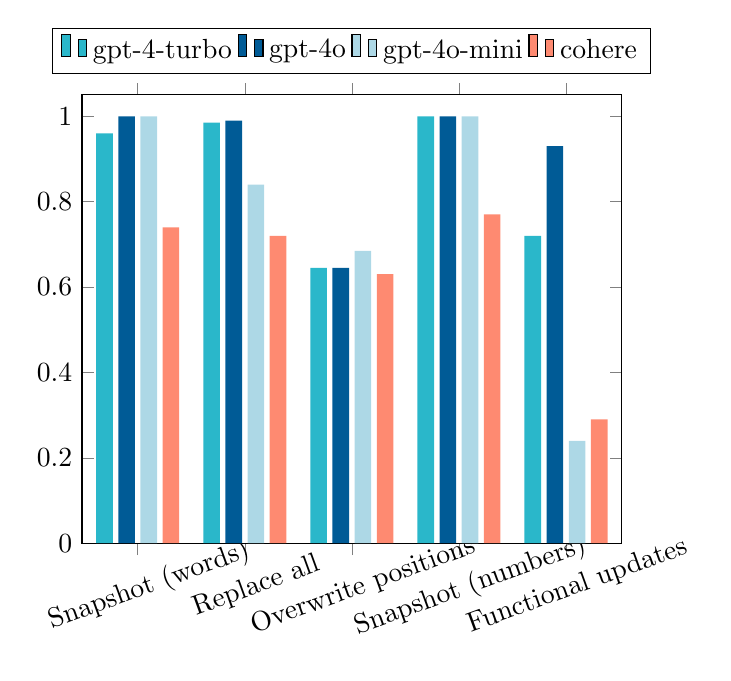
\begin{tikzpicture}
        \begin{axis}[
            ybar,
            bar width=6pt,
            symbolic x coords={Snapshot (words), Replace all, Overwrite positions, Snapshot (numbers), Functional updates},
            xtick=data,
            ymin=0, ymax=1.05,
            legend columns=4,
            legend style={at={(0.5,1.15)}, anchor=north, draw=black},
            enlarge x limits=0.13,
            xticklabel style={rotate=20, anchor=center, yshift=-12pt}
        ]
        
        \addplot[fill={rgb,255:red,42;green,183;blue,202}, draw=none] coordinates {(Snapshot (words),0.96) (Replace all,0.985) (Overwrite positions,0.645) (Snapshot (numbers),1.00) (Functional updates,0.72)};
        \addlegendentry{gpt-4-turbo}
        
        \addplot[fill={rgb,255:red,0;green,91;blue,150}, draw=none] coordinates {(Snapshot (words),1.00) (Replace all,0.99) (Overwrite positions,0.645) (Snapshot (numbers),1.00) (Functional updates,0.93)};
        \addlegendentry{gpt-4o}
        
        \addplot[fill={rgb,255:red,173;green,216;blue,230}, draw=none] coordinates {(Snapshot (words),1.00) (Replace all,0.84) (Overwrite positions,0.685) (Snapshot (numbers),1.00) (Functional updates,0.24)};
        \addlegendentry{gpt-4o-mini}
        
        \addplot[fill={rgb,255:red,254;green,138;blue,113}, draw=none] coordinates {(Snapshot (words),0.74) (Replace all,0.72) (Overwrite positions,0.63) (Snapshot (numbers),0.77) (Functional updates,0.29)};
        \addlegendentry{cohere}
        
        \end{axis}
\end{tikzpicture}}
    \end{subfigure}
    \begin{subfigure}{0.49\columnwidth}
        \resizebox{\textwidth}{!}{    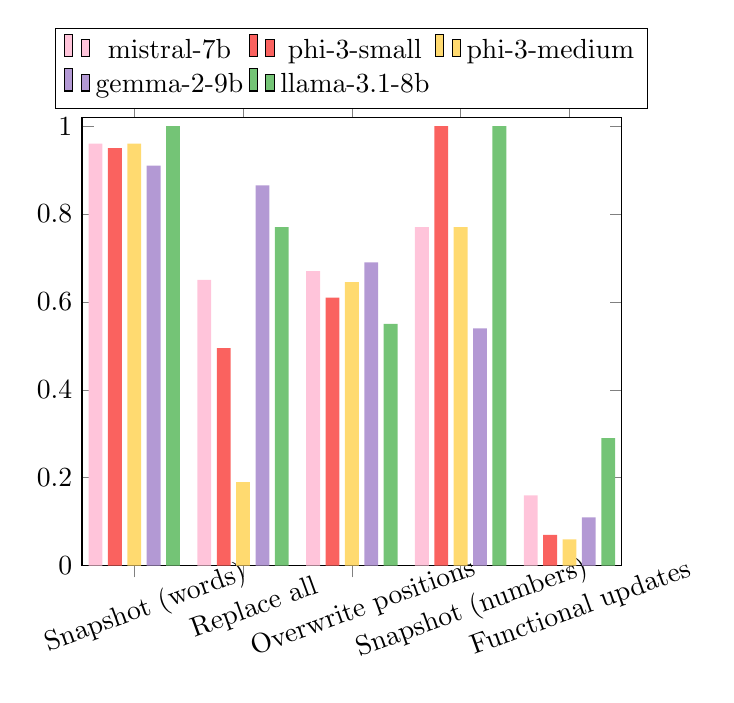
\begin{tikzpicture}
        \begin{axis}[
            ybar,
            bar width=5pt,
            symbolic x coords={Snapshot (words), Replace all, Overwrite positions, Snapshot (numbers), Functional updates},
            xtick=data,
            ymin=0, ymax=1.02,
            legend columns=3,
            legend style={at={(0.5,1.20)}, anchor=north, draw=black},
            enlarge x limits=0.12,
            xticklabel style={rotate=20, anchor=center, yshift=-12pt}
        ]
        
        \addplot[fill={rgb,255:red,255;green,196;blue,218}, draw=none] coordinates {(Snapshot (words),0.96) (Replace all,0.65) (Overwrite positions,0.67) (Snapshot (numbers),0.77) (Functional updates,0.16)};
        \addlegendentry{mistral-7b}
        
        \addplot[fill={rgb,255:red,250;green,98;blue,95}, draw=none] coordinates {(Snapshot (words),0.95) (Replace all,0.495) (Overwrite positions,0.61) (Snapshot (numbers),1.00) (Functional updates,0.07)};
        \addlegendentry{phi-3-small}
        
        \addplot[fill={rgb,255:red,255;green,218;blue,112}, draw=none] coordinates {(Snapshot (words),0.96) (Replace all,0.19) (Overwrite positions,0.645) (Snapshot (numbers),0.77) (Functional updates,0.06)};
        \addlegendentry{phi-3-medium}
        
        \addplot[fill={rgb,255:red,179;green,153;blue,212}, draw=none] coordinates {(Snapshot (words),0.91) (Replace all,0.865) (Overwrite positions,0.69) (Snapshot (numbers),0.54) (Functional updates,0.11)};
        \addlegendentry{gemma-2-9b}
        
        \addplot[fill={rgb,255:red,116;green,196;blue,118}, draw=none] coordinates {(Snapshot (words),1.00) (Replace all,0.77) (Overwrite positions,0.55) (Snapshot (numbers),1.00) (Functional updates,0.29)};
        \addlegendentry{llama-3.1-8b}
        
        \end{axis}
\end{tikzpicture}}
    \end{subfigure}
    \caption{Results for the \textbf{Recall and Edit} tasks.}
    \label{fig:recall}
\end{figure}

\paragraph{Recall and Edit} 
\begin{table}[!h]
    \centering
        \resizebox{0.8\columnwidth}{!}{%
    \begin{tabular}{lllll}
    \toprule
        \textbf{Model} & \textbf{String Search (word)} & \textbf{Snapshot} \\ \hline
gpt-4-turbo    & 1.00 \textcolor{green}{(0.06)} & 1.00 \textcolor{green}{(0.04)} \\ 
gpt-4o         & 1.00 (0.00)                   & 1.00 (0.00)                   \\ 
gpt-4o-mini    & 0.94 \textcolor{red}{(-0.04)}  & 1.00 (0.00)                   \\ 
cohere         & 1.00 (0.00)                   & 1.00 \textcolor{green}{(0.26)} \\ 
mistral-7b     & 1.00 \textcolor{green}{(0.22)} & 0.96 (0.00)                   \\ 
phi-3-small    & 1.00 \textcolor{green}{(0.06)} & 0.99 \textcolor{green}{(0.04)} \\ 
phi-3-medium   & 0.98 \textcolor{red}{(-0.02)}  & 0.87 \textcolor{red}{(-0.09)}  \\ 
gemma-2-9b     & 0.96 \textcolor{red}{(-0.04)}  & 0.96 \textcolor{green}{(0.05)} \\ 
llama-3.1-8b   & 0.98 \textcolor{red}{(-0.02)}  & 1.00 (0.00)                   \\
\bottomrule
    \end{tabular}
    }
    \caption{Ablation study with gibberish context.}
    \label{tab:ablation_gibberish}
\end{table}

Figure \ref{fig:recall} presents the results for the \textbf{Recall and Edit} tasks. While models performed well on basic recall (\textit{Snapshot}), their performance dropped sharply when tasked with making regular edits. A closer analysis of the generated outputs reveals that models struggled with maintaining coherence during edits, often getting trapped in repetitive word loops. For the \textit{Functional Update} task, we deliberately selected simple numerical updates, such as ``Subtract 1 from every number," to ensure the edits were within the models' capabilities. Nevertheless, when comparing performance on \textit{Snapshot (with numbers)} to \textit{Functional Updates}, all models exhibited a steep decline, especially for smaller ones. Analysis of generated outputs revealed that these models frequently deviated from instructions over longer sequences, suggesting difficulties in maintaining consistent rule applications over extended contexts.

Additionally, we conducted a separate ablation study on \textit{Snapshot} and \textit{String Search}. In this study, we replaced meaningful words in the context with gibberish tokens consisting of randomly generated alphabetical characters. As shown in Table \ref{tab:ablation_gibberish}, performance remained largely unchanged, suggesting that semantic meaning was not a significant distractor in these tasks.

\section{Backup: compare with previous works}

\paragraph{Comparison with Theorem 1 of \cite{srikant2024rates}.} While the framework of our proof of Theorem \ref{thm:Srikant-generalize} is mainly inspired by the proof of Theorem 1 of \cite{srikant2024rates}, there are some noteworthy differences. Most importantly, we observe that in the equation beginning from the bottom of Page 7 and continuing to the start of Page 8, the right-most side contains a term
\begin{align}\label{eq:Srikant-error}
-\frac{1}{n-k+1} \mathsf{Tr}\left(\bm{\Sigma}_{\infty}^{-\frac{1}{2}}(\bm{\Sigma}_k - \bm{\Sigma}_{\infty})\bm{\Sigma}_{\infty}^{-\frac{1}{2}}\mathbb{E}[\nabla^2 f(\tilde{\bm{Z}}_k)]\right);
\end{align}
the author argued that ``by taking an expectation to remove conditioning, and defining $\bm{A}_k$ to be $\mathbb{E}[\nabla^2 f(\tilde{\bm{Z}}_k)]$'', this term can be transformed to the term
\begin{align}\label{eq:Srikant-wrong}
-\frac{1}{n-k+1} \mathsf{Tr}\left(\bm{A}_k \left(\bm{\Sigma}_{\infty}^{-\frac{1}{2}} \mathbb{E}[\bm{\Sigma}_k]\bm{\Sigma}_{\infty}^{-\frac{1}{2}}-\bm{I}\right)\right)
\end{align}
in the expression of Theorem 1. However, we note that the function $f(\cdot)$, as defined on Page 6 as the solution to the Stein's equation with respect to $\tilde{h}(\cdot)$, is \emph{dependent on} $\mathcal{F}_{k-1}$; in fact, $f$ corresponds to the function $f_k$ in our proof. Consequently, the terms $\bm{A}_k = \mathbb{E}[\nabla^2 f(\tilde{\bm{Z}}_k)]$ (which is actually a conditional expectation with respect to $\mathcal{F}_{k-1}$), and $\bm{\Sigma}_k$ (which corresponds to $\bm{V}_k$ in our proof), are confounded by $\mathcal{F}_{k-1}$ and hence \emph{not independent}. Therefore, taking expectation, with respect to $\mathcal{F}_0$, on \eqref{eq:Srikant-error} should yield
\begin{align}\label{eq:Srikant-right}
-\frac{1}{n-k+1} \mathbb{E}\left\{\mathsf{Tr}\left(\bm{A}_k \left(\bm{\Sigma}_{\infty}^{-\frac{1}{2}} \bm{\Sigma}_k\bm{\Sigma}_{\infty}^{-\frac{1}{2}}-\bm{I}\right)\right)\right\}
\end{align}
Notice that the expectation is taken over the trace as a whole, instead of only $\bm{\Sigma}_k$. However, also due to the confounding bewteen $\bm{A}_k$ and $\bm{\Sigma}_k$, there is no guarantee that the sum of \eqref{eq:Srikant-right} is bounded as shown in the proof of Theorem 2 in \cite{srikant2024rates} on page 10. In other words, the framework of the proof needs a substantial correction to obtain a meaningful Berry-Esseen bound. 

Our solution in the proof of Theorem \ref{thm:Srikant-generalize} is to replace the matrix $\bm{Q}=\sqrt{n-k+1}\bm{\Sigma}_{\infty}$, as defined on Page 6 of \cite{srikant2024rates}, with the matrix $\bm{P}_k$, following the precedent of \cite{JMLR2019CLT}. This essentially eliminates the term \eqref{eq:Srikant-right}, but would require $\bm{P}_k$ to be measurable with respect to $\mathcal{F}_{k-1}$. For this purpose, we impose the assumption that $\bm{P}_1 = n\bm{\Sigma}_n$ almost surely, also following the precedent of \cite{JMLR2019CLT}. The relaxation of this assumption would be addressed in Theorem \ref{thm:Berry-Esseen-mtg}. 

Another important improvement we made in Theroem \ref{thm:Srikant-generalize} is to tighten the upper bound through a closer scrutiny of the smoothness of the solution to the Stein's equation, as is indicated in Proposition \ref{prop:Stein-smooth}. This paves the way for Corollary \ref{cor:Wu}, the proof of which we present in the next subsection. 


\begin{table}[!htbp] \centering
  \caption{Human Choices and Predictions About GenAI Choice in the Same Problem: Heterogeneity by Exposure and Attitudes (Pooled)}
\begin{adjustbox}{scale=0.8}
\begin{tabular}{@{\extracolsep{5pt}}lccccc}
% \\[-1.8ex]\hline
% \hline \\[-1.8ex]
\toprule
& \multicolumn{5}{c}{\textit{Dependent variable: Prediction}} \
\cr \cline{2-6}
\\[-1.8ex] & \multicolumn{1}{c}{Heavy User} & \multicolumn{1}{c}{Text-Based LLM User} & \multicolumn{1}{c}{Paid User} & \multicolumn{1}{c}{Agree AI Similar} & \multicolumn{1}{c}{Agree AI Better}  \\
\\[-1.8ex] & (1) & (2) & (3) & (4) & (5) \\
% \hline \\[-1.8ex]
\midrule
 X$\times$Heavy User & -0.056$^{}$ & & & & \\
& (0.052) & & & & \\
 X$\times$Text-Based LLM User & & 0.082$^{**}$ & & & \\
& & (0.040) & & & \\
 X$\times$Paid User & & & -0.001$^{}$ & & \\
& & & (0.072) & & \\
 X$\times$Agree AI Similar & & & & 0.033$^{}$ & \\
& & & & (0.045) & \\
 X$\times$Agree AI Better & & & & & 0.019$^{}$ \\
& & & & & (0.017) \\
 Problem FE & Yes & Yes & Yes & Yes & Yes \\
 X$\times$Problem FE & Yes & Yes & Yes & Yes & Yes \\
 G$\times$Problem FE & Yes & Yes & Yes & Yes & Yes \\
% \hline \\[-1.8ex]
\midrule
 Observations & 2700 & 2700 & 2700 & 2700 & 2700 \\
 % Residual Std. Error & 22.874 & 22.851 & 22.863 & 22.847 & 22.895 \\
% \hline
% \hline \\[-1.8ex]
\bottomrule
\textit{Note:} & \multicolumn{5}{r}{Standard errors are clustered at the problem level. $^{*}$p$<$0.1; $^{**}$p$<$0.05; $^{***}$p$<$0.01} \\
% \multicolumn{6}{r}\textit{} \\
\end{tabular}
\end{adjustbox}
\label{tab:group} \end{table}


\paragraph{Match and Compare}
 As shown in Figure \ref{fig:match}, model performance in the \textbf{Match and Compare} tasks was relatively consistent across different model sizes. Given that counting is a well-known weakness in LLMs, it is unsurprising that all models struggled significantly with the counting task, though GPT models performed slightly better than others. However, models generally succeeded in identifying the duplicates (in \textit{Find duplicates}), and primarily struggled with the counting aspect -- which requires tracking and updating an integer state, a skill that is more similar to stateful processing. This suggests that relying solely on counting-based tests \cite{song2024countingstars} could overly bias the evaluation and fail to capture broader model capabilities. The results also indicate that models exhibit some ability to recognize relative positions and group associations, but their accuracy remains limited (ranging between 0.6-0.8). A closer examination of model generations reveals an overwhelming tendency for the models to produce false positive errors -- models often answer “yes” when the correct answer is “no”, while making very few false negative errors. This means that when the relationship is correct, the models can more reliably identify it. This may stem from a combination of their inherent inclination to agree and the difficulty in recognizing relative comparisons and associations.

% \begin{figure}[h]
%     \centering
%     \includegraphics[width=0.92\columnwidth]{images/difference.png}
%     \caption{Results for \textbf{Spot the Differences }tasks.}
%     \label{fig:difference}
% \end{figure}

\begin{figure}[h]
\centering
\resizebox{0.9\columnwidth}{!}{
 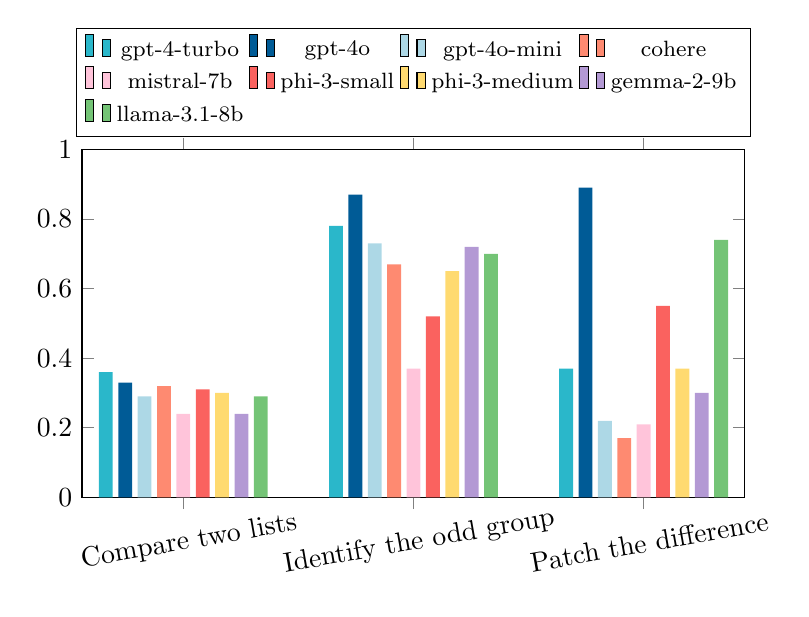
\begin{tikzpicture}
        \begin{axis}[
            ybar,
            bar width=5pt,
            symbolic x coords={Compare two lists, Identify the odd group, Patch the difference},
            xtick=data,
            ymin=0, ymax=1.0,
            legend columns=4,
            legend style={at={(0.5,1.35)}, anchor=north, draw=black, font=\footnotesize},
            enlarge x limits=0.22,
            xticklabel style={rotate=10, anchor=center, yshift=-12pt},
            width=10cm, height=6cm,
        ]
        
        \addplot[fill={rgb,255:red,42;green,183;blue,202}, draw=none] coordinates {(Compare two lists,0.36) (Identify the odd group,0.78) (Patch the difference,0.37)};
        \addlegendentry{gpt-4-turbo}
        
        \addplot[fill={rgb,255:red,0;green,91;blue,150}, draw=none] coordinates {(Compare two lists,0.33) (Identify the odd group,0.87) (Patch the difference,0.89)};
        \addlegendentry{gpt-4o}
        
        \addplot[fill={rgb,255:red,173;green,216;blue,230}, draw=none] coordinates {(Compare two lists,0.29) (Identify the odd group,0.73) (Patch the difference,0.22)};
        \addlegendentry{gpt-4o-mini}
        
        \addplot[fill={rgb,255:red,254;green,138;blue,113}, draw=none] coordinates {(Compare two lists,0.32) (Identify the odd group,0.67) (Patch the difference,0.17)};
        \addlegendentry{cohere}
        
        \addplot[fill={rgb,255:red,255;green,196;blue,218}, draw=none] coordinates {(Compare two lists,0.24) (Identify the odd group,0.37) (Patch the difference,0.21)};
        \addlegendentry{mistral-7b}
        
        \addplot[fill={rgb,255:red,250;green,98;blue,95}, draw=none] coordinates {(Compare two lists,0.31) (Identify the odd group,0.52) (Patch the difference,0.55)};
        \addlegendentry{phi-3-small}
        
        \addplot[fill={rgb,255:red,255;green,218;blue,112}, draw=none] coordinates {(Compare two lists,0.30) (Identify the odd group,0.65) (Patch the difference,0.37)};
        \addlegendentry{phi-3-medium}
        
        \addplot[fill={rgb,255:red,179;green,153;blue,212}, draw=none] coordinates {(Compare two lists,0.24) (Identify the odd group,0.72) (Patch the difference,0.30)};
        \addlegendentry{gemma-2-9b}
        
        \addplot[fill={rgb,255:red,116;green,196;blue,118}, draw=none] coordinates {(Compare two lists,0.29) (Identify the odd group,0.70) (Patch the difference,0.74)};
        \addlegendentry{llama-3.1-8b}
        
        \end{axis}
    \end{tikzpicture}}
    \caption{Results for \textbf{Spot the Differences }tasks.}
    \label{fig:difference}
\end{figure}

\paragraph{Spot the Differences}
As shown in Figure \ref{fig:difference}, performance across all models are poor on \textit{Compare Two Lists}, suggesting inherent difficulties in cross-referencing information across long contexts, even for larger models.  GPT-4o and the LLaMA model significantly outperform the others in the \textit{Identify the Odd Group} task, highlighting a general weakness in detecting contextual differences by the other models. However, an 8B LLaMA model outperforms both equivalently-sized models and even GPT-4 in this task, suggesting that model size alone was not the determining factor. This indicates that architectural differences, training objectives, or specific inductive biases may contribute to improved performance in comparative memory utilization.


\paragraph{Compute on Sets and Lists}
The tasks in this category require models to recognize and process group structures within the context, and performance gradually declines as the complexity of the task increases (see Table \ref{tab:lists}). For instance, in comparing the \textit{Group Membership} task with the \textit{String Search} task, where the former requires identifying which list a word belongs to rather than simply determining its presence, the performance of open-source models drops considerably. Similarly, in comparing the \textit{Group Association} task with the \textit{Group Membership} task, where the former requires determining whether two words belong to the same group, all models exhibit a noticeable decline in performance. The decline becomes even more pronounced when comparing the \textit{ Group Association (alternating)} variant of the task to the standard \textit{Group Association} task. Here, the context involves alternating repeated groups rather than simple group structures, which further challenges the models' abilities to handle partitioned contexts effectively.

An interesting observation was found during the \textit{Iterate} task. In an ablation study, we modified the task to require returning the first words in each list instead of the last words (making it more similar to the \textit{Batch Search} task). The performance sharply declines when models are asked to return the last words, despite their strong information-fetching capabilities. This suggests that, while the models can retrieve information effectively, they struggle to accurately recognize and process partitions within the context.


\begin{table}[h!]
\large
\centering
\begin{adjustbox}{width=\columnwidth} % Automatically fit within column width
\begin{tabular}{|c|p{0.75\columnwidth}|} % Adjust the second column width proportionally
\hline
\textbf{Symbol} & \textbf{Explanation} \\ \hline
$q^{\text{obj}} \in SE(2)$ & Object pose \\ \hline
$q^{\text{robot}} \in \mathbb{R}^9$ & Robot configuration (9 DoF robot joint position) \\ \hline
$q^{\text{obj}}_\text{sg} \in SE(2)$ & Subgoal object pose \\ \hline
$q^{\text{robot}}_\text{sg} \in SE(3) \times \mathbb{R}^3$ & Subgoal robot configuration (End-effector pose in $SE(3)$ and gripper tip positions in 3D space) \\ \hline
$q^{\text{obj}}_{\text{init}} \in SE(2)$ & Initial object pose of the task \\ \hline
$q^{\text{robot}}_{\text{init}} \in \mathbb{R}^9$ & Initial robot configuration of the task (9 DoF robot joint position) \\ \hline
$q^{\text{obj}}_{\text{goal}} \in SE(2)$ & Goal object pose of the task \\ \hline
$s$ & State \\ \hline
% $sg$ & Subgoal information (e.g., subgoal object pose, robot configuration) \\ \hline
\end{tabular}
\end{adjustbox}
\caption{Notation table for task parameters}
\label{tab:state_notation}
\end{table}

\paragraph{Stateful Processing}

\begin{figure}[t!]
    \centering
    \begin{subfigure}{0.49\columnwidth}
        \resizebox{\textwidth}{!}{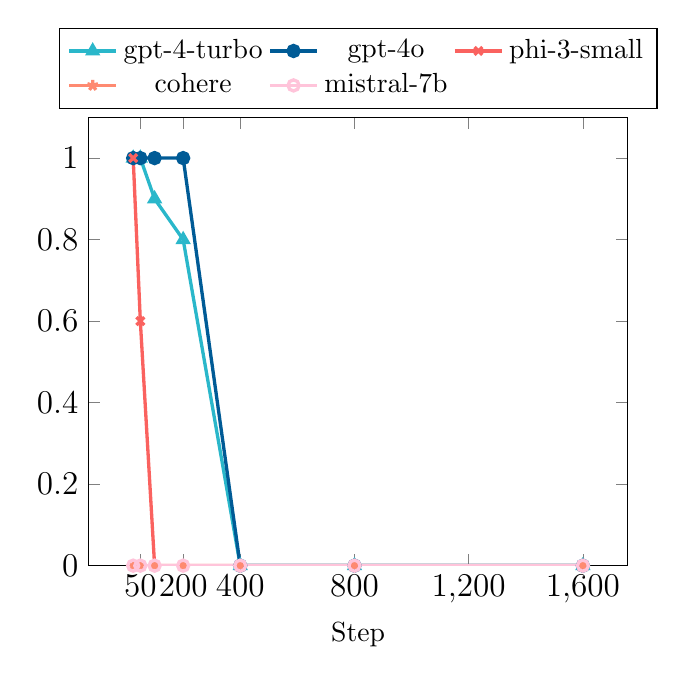
\begin{tikzpicture}
    \begin{axis}[
        xlabel={Step},
        legend style={at={(0.5,1.2)}, anchor=north, cells={align=left}, legend columns=3},
        ymin=0, ymax=1.1,
        xtick={50, 200, 400, 800, 1200, 1600},
        ytick={0,0.2,0.4,0.6,0.8,1.0},
        grid=none,
        tick label style={font=\large}
    ]

    % GPT-4-Turbo
    \addplot[mark=triangle, very thick, color={rgb,255:red,42;green,183;blue,202}] coordinates {
        (25,1.0) (50,1.0) (100,0.9) (200,0.8) (400,0.0) (800,0.0) (1600,0.0)
    };
    \addlegendentry{gpt-4-turbo}

    % GPT-4o
    \addplot[mark=*, very thick, color={rgb,255:red,0;green,91;blue,150}] coordinates {
        (25,1.0) (50,1.0) (100,1.0) (200,1.0) (400,0.0) (800,0.0) (1600,0.0)
    };
    \addlegendentry{gpt-4o}



    % Phi-3-Small
    \addplot[mark=x, very thick, color={rgb,255:red,250;green,98;blue,95}] coordinates {
        (25,1.0) (50,0.6) (100,0.0) (200,0.0) (400,0.0) (800,0.0) (1600,0.0)
    };
    \addlegendentry{phi-3-small}

    % Cohere
    \addplot[mark=star, very thick, color={rgb,255:red,254;green,138;blue,113}] coordinates {
        (25,0.0) (50,0.0) (100,0.0) (200,0.0) (400,0.0) (800,0.0) (1600,0.0)
    };
    \addlegendentry{cohere}

    % Mistral-7B
    \addplot[mark=o, very thick, color={rgb,255:red,255;green,196;blue,218}] coordinates {
        (25,0.0) (50,0.0) (100,0.0) (200,0.0) (400,0.0) (800,0.0) (1600,0.0)
    };
    \addlegendentry{mistral-7b}
    
    \end{axis}
\end{tikzpicture}}
    \end{subfigure}
    \begin{subfigure}{0.49\columnwidth}
        \resizebox{\textwidth}{!}{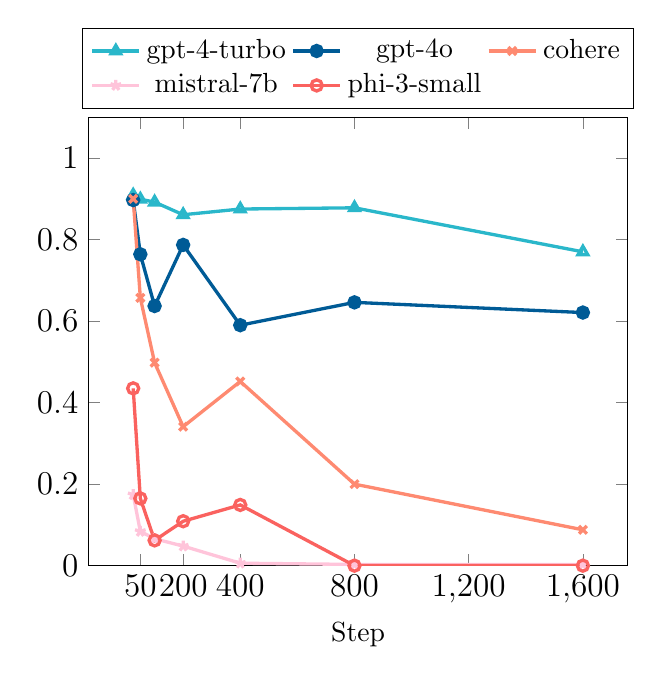
\begin{tikzpicture}
    \begin{axis}[
        xlabel={Step},
        legend style={at={(0.5,1.2)}, anchor=north, cells={align=left}, legend columns=3},
        ymin=0, ymax=1.1,
        xtick={50, 200, 400, 800, 1200, 1600},
        ytick={0,0.2,0.4,0.6,0.8,1.0},
        grid=none,
        tick label style={font=\large}
    ]

    % GPT-4-Turbo
    \addplot[mark=triangle, very thick, color={rgb,255:red,42;green,183;blue,202}] coordinates {
        (25,0.909) (50,0.899) (100,0.892) (200,0.861) (400,0.875) (800,0.878) (1600,0.770)
    };
    \addlegendentry{gpt-4-turbo}

    % GPT-4o
    \addplot[mark=*, very thick, color={rgb,255:red,0;green,91;blue,150}] coordinates {
        (25,0.897) (50,0.764) (100,0.637) (200,0.787) (400,0.590) (800,0.646) (1600,0.621)
    };
    \addlegendentry{gpt-4o}

    % Cohere
    \addplot[mark=x, very thick, color={rgb,255:red,254;green,138;blue,113}] coordinates {
        (25,0.900) (50,0.657) (100,0.498) (200,0.341) (400,0.452) (800,0.200) (1600,0.088)
    };
    \addlegendentry{cohere}

    % Mistral-7B
    \addplot[mark=star, very thick, color={rgb,255:red,255;green,196;blue,218}] coordinates {
        (25,0.174) (50,0.084) (100,0.066) (200,0.048) (400,0.006) (800,0.003) (1600,0.003)
    };
    \addlegendentry{mistral-7b}

    % Phi-3-Small
    \addplot[mark=o, very thick, color={rgb,255:red,250;green,98;blue,95}] coordinates {
        (25,0.435) (50,0.165) (100,0.062) (200,0.109) (400,0.149) (800,0.000) (1600,0.000)
    };
    \addlegendentry{phi-3-small}
    
    \end{axis}
\end{tikzpicture}}
    \end{subfigure}
    \caption{Ablation study on the number of operation steps for the \textbf{quantity state} (left) and\textbf{ set state }(right).}
    \label{fig:ablation_state_step}
\end{figure}



Table \ref{tab:state} presents the results for the \textbf{Stateful Processing} tasks, where performance gaps among models are the most pronounced. The GPT-4(o) models perform well on integer state tracking, while most other models struggle (near zero accuracy). For set state tracking, larger models generally perform better.

We conducted an ablation study to examine how the number of operation steps influences performance of five selected models (Fig. \ref{fig:ablation_state_step}). For quantity state tracking, GPT-4(o) models perform well within fewer than 200 steps but experience a sharp decline in accuracy beyond this threshold. For set state tracking, the performance decline is more gradual. The differences in performance drop between the two tasks can be attributed to the nature of the two tasks. While tracking an integer state might seem simpler than tracking a set, it actually requires the model to maintain and apply every operation sequentially to compute the final value. In contrast, for set state, the fixed size of the set makes more recent operations more relevant to the final state, reducing the need for exhaustive step-by-step tracking. Nevertheless, even in this scenario, all models show a clear inability to handle longer or more complex operation sequences effectively. Interestingly, GPT-4 model outperformed GPT-4o at this task, suggesting potential optimization trade-offs may have affected its ability to manage set-based updates. 

Overall, while larger models like GPT-4(o) exhibit some ability to track state over time, their effectiveness rapidly deteriorates as task complexity increases. Smaller models, in particular, struggle to track operations over time, pointing to significant gaps in their ability to manage and process sequential dependencies critical for state tracking tasks.

\subsection{Results on Composite Tests}

\section{Simple Construction of Projective Compositions}
\label{sec:comp_coord}

It is not clear apriori that projective compositional distributions satisfying Definition \ref{def:proj_comp} ever exist, much less that there is any straightforward way to sample from them.
To explore this, we first restrict attention to perhaps the simplest setting, where the projection functions $\{\Pi_i\}$ are
just coordinate restrictions.
This setting is meant to generalize the intuition we had
in the CLEVR example of Figure~\ref{fig:len_gen},
where different objects were composed in disjoint regions of the image.
We first define the construction of the composed distribution,
and then establish its theoretical properties.








\subsection{Defining the Construction}
Formally, suppose we have a set of distributions
$(p_1, p_2, \ldots, p_k)$ that we wish to compose;
in our running CLEVR example, each $p_i$ is the distribution of images
with a single object at position $i$.
Suppose also we have some reference distribution $p_b$,
which can be arbitrary, but should be thought of as a 
``common background'' to the $p_i$s.
Then, one popular way to construct a composed distribution
is via the \emph{compositional operator} defined below.
(A special case of this construction is used in \citet{du2023reduce}, for example).


\begin{definition}[Composition Operator]
    \label{def:comp_oper}
    Define the \emph{composition operator} $\cC$ acting on an arbitrary set of distributions $(p_b, p_1, p_2, \ldots)$ by
    \begin{align}
    \label{eq:comp_oper}
    \cC[\vec{p}] := \cC[p_b, p_1, p_2, \dots](x) := \frac{1}{Z} p_b(x) \prod_i \frac{p_i(x)}{p_b(x)},
    \end{align}
    where $Z$ is the appropriate normalization constant. We name $\cC[\vec{p}]$ the \emph{composed distribution}, and the score of $\cC[\vec{p}]$ the \emph{compositional score}:
    \begin{align}
    \label{eqn:comp_score}
    &\grad_x \log \cC[\vec{p}](x)  \\
    &= \grad_x \log p_b(x) + \sum_i \left( \grad_x \log p_i(x) - \grad_x \log p_b(x) \right). \notag
    \end{align}
\end{definition}
Notice that if $p_b$ is taken to be the unconditional distribution then this is exactly the Bayes-composition.


\vspace{-0.5em}
\subsection{When does the Composition Operator Work?}
We can always apply the composition operator to any set of distributions,
but when does this actually yield a ``correct'' composition
(according to Definition~\ref{def:proj_comp})?
One special case is when each distribution $p_i$ is
``active'' on a different, non-overlapping set of coordinates.
We formalize this property below
as \emph{Factorized Conditionals} (Definition~\ref{def:factorized}).
The idea is, 
each distribution $p_i$
must have a particular set of ``mask'' coordinates $M_i \subseteq [n]$ which it
samples in a characteristic way,
while independently sampling all other coordinates
from a common background distribution.
If a set of distributions $(p_b, p_1, p_2, \ldots)$ has this
\emph{Factorized Conditional} structure, then 
the composition
operator will produce a projective composition (as we will prove below).



\begin{definition}[Factorized-Conditionals]
\label{def:factorized}

We say a set of distributions $(p_b, p_1, p_2, \dots p_k)$
over $\R^n$
are \emph{Factorized Conditionals} if
there exists a partition of coordinates $[n]$
into disjoint subsets $M_b, M_1, \dots M_k$ such that:
\begin{enumerate}
    \setlength{\itemsep}{1pt}
    \item $(x|_{M_i}, x|_{M_i^c})$ are independent under $p_i$.
    \item $(x|_{M_b}, x|_{M_1}, x|_{M_2}, \dots, x|_{M_k})$
    are mutually independent under $p_b$.
    \item $p_i(x|_{M_i^c}) = p_b(x|_{M_i^c})$.
\end{enumerate}

Equivalently, if we have:
\begin{align}
    p_i(x) &= p_i(x|_{M_i}) p_b(x|_{M_i^c}), \text{ and} \label{eqn:cc-cond}\\
    p_b(x) &= p_b(x|_{M_b}) \prod_{i \in [k]} p_b(x|_{M_i}). \notag
\end{align}
\end{definition}
\vspace{-1em}
Equation~\eqref{eqn:cc-cond} means that each $p_i$
can be sampled by first sampling $x \sim p_b$,
and then overwriting the coordinates of $M_i$
according to some other distribution (which can be specific to distribution $i$).
For instance, the experiment of Figure~\ref{fig:len_gen}
intuitively satisfies this property, since 
each of the conditional distributions could essentially be sampled
by first sampling an empty background image ($p_b$), then ``pasting''
a random object in the appropriate location (corresponding to pixels $M_i$).
If a set of distributions obey this Factorized Conditional structure,
then we can prove that the composition operator $\cC$
yields a correct projective composition,
and reverse-diffusion correctly samples from it.
Below, let $N_t$ denote the noise operator of the
diffusion process\footnote{Our results are agnostic to the specific diffusion noise-schedule and scaling used.} at time $t$.

\begin{theorem}[Correctness of Composition]
\label{lem:compose}
Suppose a set of distributions $(p_b, p_1, p_2, \dots p_k)$
satisfy Definition~\ref{def:factorized},
with corresponding masks $\{M_i\}_i$.
Consider running the reverse-diffusion SDE 
using the following compositional scores at each time $t$:
\begin{align}
s_t(x_t) &:= \grad_x \log \cC[p_b^t, p_1^t, p_2^t, \ldots](x_t),
\end{align}
where $p_i^t := N_t[p_i]$ are the noisy distributions.
Then, the distribution of the generated sample $x_0$ at time $t=0$ is:
\begin{align}
\label{eqn:p_hat}
\hat{p}(x) := p_b(x|_{M_b}) \prod_i p_i(x|_{M_i}).
\end{align}
In particular,
$\hat{p}(x|_{M_i}) = p_i(x|_{M_i})$ for all $i$,
and so
$\hat{p}$ is a projective composition
with respect to projections $\{\Pi_i(x) := x|_{M_i}\}_i$,
per Definition \ref{def:proj_comp}.
\end{theorem}




Unpacking this, Line \ref{eqn:p_hat} says that the final generated distribution
$\hat{p}(x)$ can be sampled by
first sampling
the coordinates $M_b$ according to $p_b$ (marginally),
then independently sampling 
coordinates $M_i$ according to $p_i$ (marginally) for each $i$.
Similarly, by assumption, $p_i(x)$ can be sampled by first sampling the coordinates $M_i$ in some specific way, and then independently sampling the remaining coordinates according to $p_b$. Therefore Theorem \ref{lem:compose} says that $\hat{p}(x)$ samples the coordinates \emph{$M_i$ exactly as they would be sampled by $p_i$}, for each $i$ we wish to compose. 

\begin{proof}(Sketch) \small
Since $\vec{p}$ satisfies Definition \ref{def:factorized}, we have
\begin{align*}
&\cC[\vec{p}](x) := p_b(x) \prod_i \frac{p_i(x)}{p_b(x)} \notag 
= p_b(x) \prod_i \frac{p_b(x_t|_{M_i^c}) p_i(x|_{M_i})}{p_b(x|_{M_i^c})p_b(x|_{M_i})} \notag \\
&= p_b(x) \prod_i \frac{p_i(x|_{M_i})}{p_b(x|_{M_i})} \notag 
= p_b(x|_{M_b}) \prod_i p_i(x_t|_{M_i}) := \hat{p}(x).
\end{align*}
The sampling guarantee follows from the commutativity of composition with the diffusion noising process, i.e. $\cC[\vec{p^t}]= N_t[\cC[\vec{p}]]$. 
The complete proof is in Appendix \ref{app:compose_pf}.
\end{proof}

\begin{remark}
In fact, Theorem~\ref{lem:compose} still holds under any orthogonal transformation of the variables,
because the diffusion noise process commutes with orthogonal transforms.
We formalize this as Lemma~\ref{lem:orthogonal_sampling}.
\end{remark}

\begin{remark}
Compositionality is often thought of in terms of orthogonality between scores.
Definition \ref{def:factorized} implies orthogonality between the score differences that appear in the composed score \eqref{eqn:comp_score}:
$\grad_x \log p_i^t(x_t) - \grad_x \log p_b^t(x_t),$
but the former condition is strictly stronger
(c.f. Appendix \ref{app:score_orthog}).
\end{remark}

\begin{remark}
Notice that the composition operator $\cC$
can be applied to a set of Factorized Conditional
distributions
without knowing the coordinate partition $\{M_i\}$.
That is, we can compose distributions and compute scores
without knowing apriori exactly ``how'' these distributions are supposed to compose
(i.e. which coordinates $p_i$ is active on).
This is already somewhat remarkable, and we will see a much
stronger version of this property in the next section.
\end{remark}

\textbf{Importance of background.}
Our derivations highlight the crucial role of the background
distribution $p_b$ for the composition operator  
(Definition~\ref{def:comp_oper}).
While prior works have taken $p_b$ to be an unconditional distribution and the $p_i$'s its associated conditionals,
our results suggest this is not always the optimal choice -- in particular,
it may not satisfy a Factorized Conditional structure (Definition~\ref{def:factorized}). Figure~\ref{fig:len_gen_monster} demonstrates this empirically: settings (a) and (b) attempt to compose the same distributions using different backgrounds -- empty (a) or unconditional (b) -- with very different results.

\subsection{Approximate Factorized Conditionals in CLEVR.}
\label{sec:clevr-details}

In \cref{fig:len_gen_monster} we explore compositional length-generalization (or lack thereof) in three different setting, two of which (\cref{fig:len_gen_monster}a and \ref{fig:len_gen_monster}c) approximately satisfy \cref{def:factorized}. In this section we explicitly describe how our definition of Factorized Conditionals approximately captures the CLEVR settings of Figures \ref{fig:len_gen_monster}a and \ref{fig:len_gen_monster}c. The setting of \ref{fig:len_gen_monster}b does not satisfy our conditions, as discussed in \cref{sec:problematic-compositions}.

\textbf{Single object distributions with empty background.}
This is the setting of both \cref{fig:len_gen} and \cref{fig:len_gen_monster}a.
The background distribution $p_b$ 
over $n$ pixels is images of an empty scene with no objects.
For each $i \in \{1,\ldots,L\}$ (where $L=4$ in \cref{fig:len_gen} and $L=9$ in \cref{fig:len_gen_monster}a), define the set $M_i \subset [n]$ 
as the set of pixel indices surrounding location $i$.
($M_i$ should be thought of as a ``mask'' that
that masks out objects at location $i$).
Let $M_b := (\cup_i M_i)^c$ be the remaining
pixels in the image.
Then, we claim the distributions $(p_b, p_1, \ldots, p_L)$
form approximately
Factorized Conditionals, with corresponding
coordinate partition $\{M_i\}$.
This is essentially because each distribution $p_i$
matches the background $p_b$ on all pixels except those surrounding
location $i$ (further detail in Appendix~\ref{app:clevr-details}).
Note, however, that the conditions of Definition~\ref{def:factorized}
do not \emph{exactly} hold in the experiment of Figure~\ref{fig:len_gen} -- there is still some dependence between
the masks $M_i$, since objects can cast shadows or even occlude each other.
Empirically, these deviations 
have greater impact
when composing many objects, as seen in \cref{fig:len_gen_monster}a.


\textbf{Bayes composition with cluttered distributions.}
In \cref{fig:len_gen_monster}c we replicate CLEVR experiments in  \citet{du2023reduce, liu2022compositional} where the images contain many objects (1-5) and the conditions label the location of one randomly-chosen object. It turns out the unconditional together with the conditionals can approximately act as Factorized Conditionals in ``cluttered'' settings like this one. The intuition is that if the conditional distributions each contain one specific object plus many independently sampled random objects (``clutter''), then the unconditional distribution \emph{almost} looks like independently sampled random objects, which together with the conditionals \emph{would} satisfy Definition \ref{def:factorized} (further discussion in Appendix \ref{app:clevr-details} and \ref{app:bayes_connect}). This helps to explain the length-generalization observed in \citet{liu2022compositional} and verified in our experiments (\cref{fig:len_gen_monster}c).







\section{Projective Composition in Feature Space}
\label{sec:comp_feature}

\begin{figure}
    \centering
    \includegraphics[width=1.0\linewidth]{figures/feat-space-vis.png}
    \caption{A commutative diagram illustrating Theorem~\ref{lem:transform_comp}.
    Performing composition in pixel space is equivalent 
    to encoding into a feature space ($\cA$),
    composing there,
    and decoding back
    to pixel space ($\cA^{-1}$).
    }
    \label{fig:feat-space-vis}
\end{figure}

So far we have focused on the setting where the projection functions $\Pi_i$ are simply projections onto coordinate subsets $M_i$ in the native space (e.g. pixel space).
This covers simple examples like Figure~\ref{fig:len_gen} but does not include more realistic situations such as Figure~\ref{fig:style-content},
where the properties to be composed are more abstract.
For example a property like ``oil painting'' does not correspond to projection
onto a specific subset of pixels in an image.
However, we may hope that there exists some conceptual feature space
in which ``oil painting'' does correspond to a particular subset of variables.
In this section, we extend our results to the case where the composition occurs in some conceptual feature space, and each distribution to be composed
corresponds to some particular subset of \emph{features}.


Our main result is a featurized analogue of Theorem~\ref{lem:compose}:
if there exists \emph{any} invertible transform $\cA$
mapping into a feature space
where Definition \ref{def:factorized} holds,
then the composition operator (Definition~\ref{def:comp_oper})
yields a projective composition in this feature space, as shown in Figure~\ref{fig:feat-space-vis}.

\begin{theorem}[Feature-space Composition]
\label{lem:transform_comp}
Given distributions $\vec{p} := (p_b, p_1, p_2, \dots p_k)$,
suppose there exists a diffeomorphism $\cA: \R^n \to \R^n$
such that
$(\cA \sharp p_b, \cA \sharp p_1, \dots \cA \sharp p_k)$
satisfy Definition~\ref{def:factorized},
with corresponding partition $M_i \subseteq [n]$.
Then, the composition $\hat{p} := \cC[\vec{p}]$ satisfies:
\begin{align}
\label{eqn:p_hat_A}
\cA \sharp \hat{p}(z)
\equiv
(\cA \sharp p_b (z))|_{M_b} \prod_{i=1}^k (\cA \sharp p_i(z))|_{M_i}.
\end{align}
Therefore, $\hat{p}$
is a projective composition of $\vec{p}$ w.r.t. projection functions
$\{\Pi_i(x) := \cA(x)|_{M_i}\}$.
\end{theorem}
This theorem is remarkable because it means we can
compose distributions $(p_b, p_1, p_2, \dots)$ in the base space,
and this composition will ``work correctly'' in the feature space
automatically (Equation~\ref{eqn:p_hat_A}),
without us ever needing to compute or even know the feature transform $\cA$
explicitly.



Theorem~\ref{lem:transform_comp} may apriori seem too strong
to be true, since it somehow holds for all feature spaces $\cA$
simultaneously.
The key observation underlying Theorem~\ref{lem:transform_comp} 
is that the composition operator $\cC$ behaves
well under reparameterization.
\begin{lemma}[Reparameterization Equivariance]
\label{lem:reparam}
The composition operator of Definition~\ref{def:comp_oper}
is reparameterization-equivariant. That is,
for all diffeomorphisms $\cA: \R^n \to \R^n$
and all tuples of distributions $\vec{p} = (p_b, p_1, p_2, \dots, p_k)$,
\begin{align}
 \cC[ \cA \sharp \vec{p}] =  \cA \sharp \cC[\vec{p}].
\end{align}
\end{lemma}
\arxiv{\footnote{
For example (separate from our goals in this paper):
Classifier-Free-Guidance can be seen as an instance of the composition operator.
Thus, Lemma~\ref{lem:reparam} implies that performing CFG
in latent space is \emph{equivalent} to CFG in pixel-space,
assuming accurate score-models in both cases.}}
\arxiv{This lemma is potentially of independent interest:
reparametrization-equivariance
is a very strong property which is typically not satisfied by
standard operations between probability distributions---
for example, the ``simple product'' $p_1(x)p_2(x)$ does not satisfy it---
so it is mathematically notable that the composition operator 
has this structure.
Lemma~\ref{lem:reparam} and Theorem~\ref{lem:transform_comp}
are proved in Appendix \ref{app:param-indep}.}

This lemma is potentially of independent interest:
equivariance distinguishes the composition operator
from many other common operators
(e.g. the simple product).
Lemma ~\ref{lem:reparam} and Theorem~\ref{lem:transform_comp}
are proved in Appendix \ref{app:param-indep}.

\section{Sampling from Compositions.}
The feature-space Theorem~\ref{lem:transform_comp} is weaker than Theorem~\ref{lem:compose}
in one important way: it does not provide a sampling algorithm.
That is, Theorem~\ref{lem:transform_comp} guarantees that $\hat{p} := \cC[\vec{p}]$
is a projective composition, but does not guarantee that reverse-diffusion
is a valid sampling method.

There is one special case where diffusion sampling \emph{is} guaranteed to work, namely, for orthogonal transforms (which can seen as a straightforward extension of the coordinate-aligned case of \cref{lem:compose}):
\begin{lemma}[Orthogonal transform enables diffusion sampling]
\label{lem:orthogonal_sampling}
If the assumptions of Lemma \ref{lem:transform_comp} hold for $\cA(x) = Ax$, where $A$ is an orthogonal matrix, then running a reverse diffusion sampler with scores $s_t = \grad_x \log \cC[\vec{p}^t]$ generates the composed distribution $\hat{p} = \cC[\vec{p}]$ satisfying \eqref{eqn:p_hat_A}.
\end{lemma}
The proof is given in \cref{app:orthog_sample_pf}.

However, for general invertible transforms, we have no such sampling guarantees.
Part of this is inherent: in the feature-space setting, the 
diffusion noise operator $N_t$ no longer commutes
with the composition operator $\cC$ in general,
 so scores of the noisy composed 
distribution $N_t[\cC[\vec{p}]]$
cannot be computed from scores
of the noisy base distributions $N_t[\vec{p}]$.
Nevertheless, one may hope to sample from the distribution $\hat{p}$
using other samplers besides diffusion, 
such as annealed Langevin Dynamics
or
Predictor-Corrector methods \citep{song2020score}.
We find that the situation is surprisingly subtle:
composition $\cC$ produces distributions which
are in some cases easy to sample (e.g. with diffusion),
yet in other cases apparently hard to sample.
For example, in the
setting of Figure~\ref{fig:clevr_color_comp}, 
our Theorem~\ref{lem:transform_comp} implies
that all pairs of colors should compose equally well
at time $t=0$, since there exist diffeomorphisms
(indeed, linear transforms) between different colors.
However, as we saw,
the diffusion sampler
fails to sample from compositions 
of non-orthogonal colors--- and 
empirically, even more sophisticated
samplers such as Predictor-Correctors
also fail in this setting.
At first glance, it may seem odd that
composed distributions are so hard to sample,
when their constituent distributions are relatively easy to sample.
One possible reason for this below is that the composition operator has extremely poor Lipchitz constant,
so it is possible for a set of distributions $\vec{p}$ to ``vary smoothly''
(e.g. diffusing over time) while their composition $\cC[\vec{p}]$
changes abruptly.
We formalize this in \cref{lem:lipschitz} (further discussion and proof in Appendix \ref{app:lipschitz}).
\begin{lemma}[Composition Non-Smoothness]
\label{lem:lipschitz}
For any set of distributions $\{p_b, p_1, p_2, \dots, p_k\}$,
and any noise scale $t := \sigma$,
define the noisy distributions 
$p_i^t := N_{t}[p_i]$,
and let $q^t$ denote the composed distribution at time $t$: $q^t := \cC[\vec{p}^t]$. Then, for any choice of $\tau > 0$,
there exist distributions $\{p_b, p_1, \dots p_k\}$ over $\R^n$
such that
\begin{enumerate}
    \setlength{\itemsep}{0pt}
    \item For all $i$, the annealing path of $p_i$ is 
    $\cO(1)$-Lipshitz:
    $\forall t, t': W_2(p_i^{t}, p_i^{t'}) \leq \cO(1) |t - t'|$.
    \item The annealing path of $q$ has Lipshitz constant
    at least $\Omega(\tau^{-1})$:
    $\exists t, t': W_2(q^{t}, q^{t'}) \geq \frac{|t - t'|}{2\tau}.$
\end{enumerate}
\end{lemma}




The composite tests significantly challenge the models by combining multiple atomic capabilities into a single test. In the \textit{Processing Data Blocks} task, the context is fixed at 4k tokens, while for the \textit{Theory of Mind} task, the number of operation steps is set to 100. As shown in Table \ref{tab:comp}, model performance on both tasks are generally low, showing a broad inability to handle the more complex scenarios. Performance across all models drop substantially on composite tasks compared to their performance on individual capability tasks, such as search, recall, and group processing. 

Interestingly, some smaller models, like Mistral and Phi-3-small, exhibit slightly better performance on the \textit{Theory of Mind} task than on the set state tracking task. This anomaly likely stems from their already weak state tracking ability, which limits their performance across both tasks. Additionally, these models tend to generate longer answers in the set state task which reduces the set overlap.

Notably, even the most capable models, such as GPT-4-turbo and GPT-4o, struggle, showing that scaling model size alone is not enough for solving these composite tasks. Additionally, the variation in performance among smaller models suggests that their limitations stem not only from size but also from underlying architectural or training differences. This indicates that smaller models require more targeted care to bridge the gap in effective memory use.



\section{Downstream Tasks}
\label{sec:downstream_tasks}
In this section, we show the effectiveness of the Wizard-of-Shopping dataset by applying it to two downstream tasks: Conversational Query Generation (CQG) and Conversational Product Ranking (CPR). For both tasks, we divided the \textit{WoS} conversations into 3,000 for training, 300 for validation, and 300 for testing, with each split containing an equal number of dialogues from the three domains. More details are available in Appendix \ref{sec:detailed_downstream_tasks}.

\subsection{Conversational Query Generation (CQG)}

Real product search conversations are likely to be verbose and redundant for the purpose of product ranking.  
Similar to the conversational search~\cite{yu2020few,vakulenko2021question,chen-etal-2022-reinforced,wu2022conqrr} where a reformulation model is used to generate a more informative query from the dialogue history, we address \textit{conversational query generation} (CQG) for product search. 
CQG aims to extract essential information such as the product category under discussion, desired features, undesired features, and optional product preferences from the customer. This extracted information can then be used as a query for a product search engine. And in fact, this is a reverse task of the LLM verbalization where we extract user preferences from the shopping dialogues. Similar to Dialogue State Tracking~\cite{lu2023dialgen}, CQG is helpful in tracing the interest of customers during the conversation. 
%can be extracted for product ranking and DST while the conversation is in progress.
%As the reverse task of the LLM verbalization, the CQG task condenses a long shopping conversation into a structured form that encodes the most essential information about conversational product search. %\shervin{What is the purpose of the task? what is it used for?} 
As \citet{bi2019conversational} suggests, utilizing positive and negative product features are crucial for training a conversational product ranking model. We train a conversational query generator on the \textit{WoS} data to extract the product category and the customer-preferred product features:
%\begin{equation*}
%\vspace{-1em}
\begin{equation}\label{eq:cqg}  \small
    [PC, Wanted, Unwanted, Optional] \gets CQG(Dialogue)
\end{equation}
\vspace{-2em}
%\hl{Jason: is this input same to preference?} % Xiangci: Yes.



\subsubsection{Approaches} \label{sec:conversational_query_generation_approaches}

\paragraph{Baseline.} As stated in \S\ref{sec:related_work}, to the best of our knowledge, \textit{WoS} is the only CPS dataset that can be used for training downstream tasks. Therefore as a simple baseline, we directly use the full conversation history as the predicted query.
%\vspace{-0.5em}
\paragraph{Dialogue --> Query (D2Q).} We use a seq2seq model, Longformer Encoder-Decoder \citep[LED;][]{beltagy2020longformer} fine-tuned on our \textit{WoS} dataset to predict the product category and the \textit{wanted}, \textit{unwanted} and \textit{optional} product features, given the full conversation history.

\paragraph{D2Q (GPT-4).} For reference of LLM performance, we few-shot prompt OpenAI gpt-4-turbo-2024-04-09 with the same inputs and outputs as D2Q.
%\paragraph{Utterance-level.} We assume that each utterance between the seller and customer encodes one or more product features. We use a seq2seq model to extract product features from each utterance, and concatenate the features to be the final query.

% \begin{table}[t]  \small
% \centering
% \setlength{\tabcolsep}{4pt}
% \begin{tabular}{lllllll}
% \hline
% \textbf{Approach} & \textbf{Features} & \textbf{F1} & \textbf{R-1} & \textbf{R-2} & \textbf{R-L}\\ \hline
% Baseline & + & 0 & 0.056 & 0.020 & 0.048 \\ 
% Baseline & +/-/? & 0.008 & 0.137 & 0.047 & 0.087  \\  \hline 
% %Utterance & BART & + & 0.698 & 0.592 & 0.482 & 0.562 \\ 
% %Utterance & BART & +/-/? & 0.656 & 0.664 & 0.489 & 0.592 \\  \hline
% %Utterance & LED & + & 0.704 & 0.610 & 0.509 & 0.578 \\ 
% %Utterance & LED & +/-/? & 0.748 & 0.720 & 0.561 & 0.657 \\  \hline
% D2Q & + & 0.834 & 0.899 & 0.822 & 0.873 \\ 
% D2Q & +/-/? & 0.873 & 0.900 & 0.768 & 0.840 \\  \hline
% \end{tabular}
% \vspace{-0.5em}
% \caption{Conversational Query Generation performance at the final turn measured by exact-F1, ROUGE-1, -2, and -L. We report the performance of only using the desired features (+) for downstream ranking, as well as using all features (wanted (+), unwanted (-), and optional (?)).}
% \label{tab:conversational_query_generation}
% \vspace{-2em}
% \end{table}

\begin{table}[t]  \small
\centering
\setlength{\tabcolsep}{4pt}
\begin{tabular}{llllll}
\hline
\textbf{Approach} & \textbf{F1} & \textbf{R-1} & \textbf{R-2} & \textbf{R-L}\\ \hline
%Baseline & 0 & 0.056 & 0.020 & 0.048 \\ 
Baseline & 0.008 & 0.137 & 0.047 & 0.087  \\  \hline  
%Utterance & BART & + & 0.698 & 0.592 & 0.482 & 0.562 \\ 
%Utterance & BART & +/-/? & 0.656 & 0.664 & 0.489 & 0.592 \\  \hline
%Utterance & LED & + & 0.704 & 0.610 & 0.509 & 0.578 \\ 
%Utterance & LED & +/-/? & 0.748 & 0.720 & 0.561 & 0.657 \\  \hline
D2Q & 0.834 & 0.899 & 0.822 & 0.873 \\ \hline
D2Q (GPT-4) & 0.553 & 0.793 & 0.628 & 0.734 \\ \hline
%D2Q & +/-/? & 0.873 & 0.900 & 0.768 & 0.840 \\  \hline
\end{tabular}
\vspace{-0.5em}
\caption{Conversational Query Generation performance at the final turn measured by exact-F1, ROUGE-1, -2, and -L.}
\label{tab:conversational_query_generation}
\vspace{-2em}
\end{table}

\subsubsection{Experimental Results}
Table \ref{tab:conversational_query_generation} shows the performance of the CQG task.
%We report results on two settings: \textit{wanted} feature-only setups concatenate the product category and \textit{wanted} features and all feature setups concatenate all features as defined in Eq.~\ref{eq:cqg}. 
As expected, the weak baseline using conversation history performs poorly, while our fine-tuned query generator performs much better. %Additionally, we observe that predicting product features utterance-by-utterance instead underperforms using the full conversation (\S\ref{sec:detailed_conversational_query_generation} \& Table \ref{tab:detailed_conversational_query_generation}), which is consistent with prior work of reformulating conversations into queries \cite{yu2020few, wu2022conqrr}. 
Although GPT-4's performance is slightly underestimated because few-shot demonstration examples do not show every edge case, D2Q by \textit{WoS}-finetuned LED shows its superiority of both performance and cost in terms of both latency and price over GPT-4 as an example of LLM.
%When comparing the utterance-level approaches, LED outperforms BART, since the training data for BART is slightly smaller than LED's. This is because we have to discard the input augmented conversation history that is too long for BART's maximum context window (1024 tokens). Also, the LED-based utterance level approach under-performs the conversation level approach, presumably because integrating the results from multiple inferences passes is more error-prone. 

\subsection{Conversational Product Ranking (CPR)}
As the core component of CPS, CPR directly ranks the candidate products given the shopping conversation. We index or embed each product's title and concatenate their aspect-value pairs according to the following approaches:

\subsubsection{Approaches}%\zhiyu{Define what is indexed for each document/product. Title ? Description ?}

\paragraph{Baseline} %Similar to the CQG task, we assume there is no conversational data available for training a ranker. Therefore, w
We directly feed the full conversation history as the query to a BM25 ranker.

%\paragraph{Dialogue --> Product (D2P)} We directly embed the full conversation history to a dense ranker to rank the candidate products, i.e. \textit{Products = Ranker(Dialogue)}. %\zhiyu{related to my previous comments. If products are ranked by Relevance = Ranker(dialogue, product\_info), what is product\_info here?}
\vspace{-0.5em}
\paragraph{Dialogue --> Query --> Product (D2Q2P)} We use D2Q setting in \S\ref{sec:conversational_query_generation_approaches} to generate queries given the full conversation history and apply the queries to a ranker, i.e. \textit{Products = Ranker(CQG(Dialogue))}. We experiment with both a sparse ranker, BM25, and a dense ranker \citep[fine-tuned RoBERTa;][]{liu2019roberta}.

\paragraph{D2Q2P (GPT-4)} We use D2Q (GPT-4) setting in \S\ref{sec:conversational_query_generation_approaches} and feed the predicted query to a BM25 ranker.

\begin{table}[t]  \small
\centering
\setlength{\tabcolsep}{2pt} % Default value: 6pt
\renewcommand{\arraystretch}{1.0} % Default value: 1
\begin{tabular}{llllllll}
\hline
\textbf{Approach} & \textbf{Ranker} & \textbf{MRR} & \textbf{H@1} & \textbf{H@10} & \textbf{H@100}\\ \hline
Baseline & BM25& 0.162 & 0.107 & 0.203 & 0.587 \\ \hline \hline
%D2P & - & longformer & 0.201 & 0.143  & 0.247 & 0.620 \\ \hline
%Utterance & BART & BM25& 0.629 & 0.540  & 0.733 & 0.900 \\
%Utterance & BART & Roberta& 0.217 & 0.163 & 0.270 & 0.477\\ \hline
%Utterance & LED & BM25& 0.667 & 0.593 & 0.740 & 0.900 \\
%Utterance & LED & Roberta& 0.207 & 0.163 & 0.250 & 0.460 \\ \hline
D2Q2P & BM25& \textbf{0.838} & \textbf{0.767}  & \textbf{0.927} & \textbf{0.993} \\
D2Q2P & Roberta & 0.675 & 0.583  & 0.780 & 0.937 \\ \hline
D2Q2P (GPT-4) & BM25 & 0.763 & 0.680 & 0.903 & 0.903 \\ \hline 

\end{tabular}
\vspace{-0.5em}
\caption{Downstream CPR performance at the final turn.}
\label{tab:ranker}
\vspace{-2em}
\end{table}

\subsubsection{Experimental Results}
Table \ref{tab:ranker} shows the mean reciprocal rank (MRR) and Hit$@k$ of all methods. 
%We observe that the D2P approach only slightly outperforms the baseline approach without training. We suspect that our DPR-Longformer is still under-fitted given 3000 conversations as the training set. On the contrary, by leveraging the query generators trained on our collected conversations, the ranking performance is greatly improved. 
%Similar to the trend observed in the conversational query generation task, the conversation-level approach outperforms the utterance-level approach that integrates multiple passes of inference outputs. 
Similar to the trend observed for CQG, our D2Q2P approach significantly outperforms the baseline and GPT-4. Interestingly, the sparse BM25 ranker greatly outperforms the dense RoBERTa-based ranker. This is because the product representations include feature names that are lexically similar to the gold queries. Consequently, BM25 exhibits a strong performance in this ranking task. Moreover, the dense ranker may be under-fitted. The query generators and dense rankers fine-tuned on our \textit{WoS} dataset significantly outperform the baseline that is not trained on our dataset.


\section{Conclusions}
We propose a method, \method, to automatically generate target-oriented shopping conversations without any human annotations. 
% Unlike prior work that learns various user or item representations, \method adds a conversation layer on top of the traditional product search to achieve CPS. 
We leverage decision tree to explore the vast product search space, and construct a dialogue plan that minimizes the number of search steps required to retrieve a relevant product.
%We then successfully compute a dialogue plan that is suitable for feeding into LLMs as prompts, and that guarantees the success of product search with the fewest product features to be clarified.
The resulting corpus (\textit{WoS}), generated using single-pass approach with GPT-4, not only achieved highly natural (4.2/5.0) and coherent (4.7/5.0) ratings from human annotators, but also showed substantial improvements when applied to two downstream tasks. By releasing our dataset and approach, we hope to expedite the research and development of intelligent CPS systems in future.

%We further improve the naturalness of our generated conversations through carefully curated prompts, dynamically listing example product values and leveraging the internal knowledge of the LLMs. We use \method's single pass generation technique with GPT-4 to create and release the \textit{Wizard-of-Shopping} (\textit{WoS}) dataset. Human evaluation shows it is sufficiently natural. Finally, we utilize \textit{WoS} to fine-tune models for downstream CQG and CPR tasks, and find that they significantly outperform baselines not trained on our dialogue dataset. %without using our dataset for training. Therefore, we conclude that our collected CPS dataset can effectively improve the downstream tasks.


\section*{Limitations}
%\subsection{Limitations}
Despite the demonstrated potential of our \method approach and the \textit{WoS} dataset, there are still some limitations that we leave for future work. %\jason{maybe we should work on summarizing all these restrictions. We definitely should discuss limitations, but not sure it is the best place to enumerate all at the last paragraph of our paper. Maybe create a separate section called limitation on section 6?} 
%First, the diversity of our conversations is still insufficient. We find that high-performing LLMs including GPT-4 are not sensitive to instructions regarding \textit{customer persona} (e.g., customer patience, expertise level). Thus, there is no distinction between multiple customers across conversations other than search behavior preferences. 
%Next, \textit{WoS} conversations are all target-oriented with a similar conversation flow -- starting with stating the target product category, identifying the product feature requirements, and finally recommending a qualifying product to the customer. Consequently, 
First, \method does not consider more complicated shopping behavior such as comparison among similar products~\cite{vedula2022matters}. %, or allowing customers to change their mind and roll back to a previous state. 
In the future, we could extend the ability of \method and allow customers to choose a similar product in the search results for comparison with assistance from a LLM agent. 
Second, the quality of \textit{WoS} conversations relies on the quality of the product catalog. Since noise in the product catalog can directly propagate to the generated conversations. Methods proposed to curate and clean the product catalog~\cite{ghani2006text,yang2022mave,vedula2022matters} could be applied to further clean a product catalog. %Moreover, the vocabulary size \jason{this seems redundant. in different places you already talk about the OOV problem} of the product features may directly affect the diversity of the conversation, as well as the feasibility of using the interactive system as a virtual shopping assistant. 
Finally, since the decision tree treats every product aspect and value as a categorical label, the semantics of product features are under-utilized. Future work may further leverage the zero-shot ability of LLMs to mine the semantics of the product aspects, so that similar product features may be merged to produce a more natural and efficient dialogue plan.

\section*{Ethical Statements}
The potential risk of our work could be biased simulations of real-world users' behavior, such that the learned downstream CQG and CPR models are biased. As a result, the end user's will of shopping might be distorted by the CPS system. However, we note that this risk is hypothetical.
\clearpage
%\bibliography{anthology,custom}
\bibliography{sample-base}
\bibliographystyle{acl_natbib}
\clearpage
\appendix
\section{Secure Token Pruning Protocols}
\label{app:a}
We detail the encrypted token pruning protocols $\Pi_{prune}$ in Figure \ref{fig:protocol-prune} and $\Pi_{mask}$ in Figure \ref{fig:protocol-mask} in this section.

%Optionally include supplemental material (complete proofs, additional experiments and plots) in appendix.
%All such materials \textbf{SHOULD be included in the main submission.}
\begin{figure}[h]
%vspace{-0.2in}
\begin{protocolbox}
\noindent
\textbf{Parties:} Server $P_0$, Client $P_1$.

\textbf{Input:} $P_0$ and $P_1$ holds $\{ \left \langle Att \right \rangle_{0}^{h}, \left \langle Att \right \rangle_{1}^{h}\}_{h=0}^{H-1} \in \mathbb{Z}_{2^{\ell}}^{n\times n}$ and $\left \langle x \right \rangle_{0}, \left \langle x \right \rangle_{1} \in \mathbb{Z}_{2^{\ell}}^{n\times D}$ respectively, where H is the number of heads, n is the number of input tokens and D is the embedding dimension of tokens. Additionally, $P_1$ holds a threshold $\theta \in \mathbb{Z}_{2^{\ell}}$.

\textbf{Output:} $P_0$ and $P_1$ get $\left \langle y \right \rangle_{0}, \left \langle y \right \rangle_{1} \in \mathbb{Z}_{2^{\ell}}^{n'\times D}$, respectively, where $y=\mathsf{Prune}(x)$ and $n'$ is the number of remaining tokens.

\noindent\rule{13.2cm}{0.1pt} % This creates the horizontal line
\textbf{Protocol:}
\begin{enumerate}[label=\arabic*:, leftmargin=*]
    \item For $h \in [H]$, $P_0$ and $P_1$ compute locally with input $\left \langle Att \right \rangle^{h}$, and learn the importance score in each head $\left \langle s \right \rangle^{h} \in \mathbb{Z}_{2^{\ell}}^{n} $, where $\left \langle s \right \rangle^{h}[j] = \frac{1}{n} \sum_{i=0}^{n-1} \left \langle Att \right \rangle^{h}[i,j]$.
    \item $P_0$ and $P_1$ compute locally with input $\{ \left \langle s \right \rangle^{i} \in \mathbb{Z}_{2^{\ell}}^{n}  \}_{i=0}^{H-1}$, and learn the final importance score $\left \langle S \right \rangle \in \mathbb{Z}_{2^{\ell}}^{n}$ for each token, where  $\left \langle S \right \rangle[i] = \frac{1}{H} \sum_{h=0}^{H-1} \left \langle s \right \rangle^{h}[i]$.
    \item  For $i \in [n]$, $P_0$ and $P_1$ invoke $\Pi_{CMP}$ with inputs  $\left \langle S \right \rangle$ and $ \theta $, and learn  $\left \langle M \right \rangle \in \mathbb{Z}_{2^{\ell}}^{n}$, such that$\left \langle M \right \rangle[i] = \Pi_{CMP}(\left \langle S \right \rangle[i] - \theta) $, where: \\
    $M[i] = \begin{cases}
        1  &\text{if}\ S[i] > \theta, \\
        0  &\text{otherwise}.
            \end{cases} $
    % \item If the pruning location is insensitive, $P_0$ and $P_1$ learn real mask $M$ instead of shares $\left \langle M \right \rangle$. $P_0$ and $P_1$ compute $\left \langle y \right \rangle$ with input $\left \langle x \right \rangle$ and $M$, where  $\left \langle x \right \rangle[i]$ is pruned if $M[i]$ is $0$.
    \item $P_0$ and $P_1$ invoke $\Pi_{mask}$ with inputs  $\left \langle x \right \rangle$ and pruning mask $\left \langle M \right \rangle$, and set outputs as $\left \langle y \right \rangle$.
\end{enumerate}
\end{protocolbox}
\setlength{\abovecaptionskip}{-1pt} % Reduces space above the caption
\caption{Secure Token Pruning Protocol $\Pi_{prune}$.}
\label{fig:protocol-prune}
\end{figure}




\begin{figure}[h]
\begin{protocolbox}
\noindent
\textbf{Parties:} Server $P_0$, Client $P_1$.

\textbf{Input:} $P_0$ and $P_1$ hold $\left \langle x \right \rangle_{0}, \left \langle x \right \rangle_{1} \in \mathbb{Z}_{2^{\ell}}^{n\times D}$ and  $\left \langle M \right \rangle_{0}, \left \langle M \right \rangle_{1} \in \mathbb{Z}_{2^{\ell}}^{n}$, respectively, where n is the number of input tokens and D is the embedding dimension of tokens.

\textbf{Output:} $P_0$ and $P_1$ get $\left \langle y \right \rangle_{0}, \left \langle y \right \rangle_{1} \in \mathbb{Z}_{2^{\ell}}^{n'\times D}$, respectively, where $y=\mathsf{Prune}(x)$ and $n'$ is the number of remaining tokens.

\noindent\rule{13.2cm}{0.1pt} % This creates the horizontal line
\textbf{Protocol:}
\begin{enumerate}[label=\arabic*:, leftmargin=*]
    \item For $i \in [n]$, $P_0$ and $P_1$ set $\left \langle M \right \rangle$ to the MSB of $\left \langle x \right \rangle$ and learn the masked tokens $\left \langle \Bar{x} \right \rangle \in Z_{2^{\ell}}^{n\times D}$, where
    $\left \langle \Bar{x}[i] \right \rangle = \left \langle x[i] \right \rangle + (\left \langle M[i] \right \rangle << f)$ and $f$ is the fixed-point precision.
    \item $P_0$ and $P_1$ compute the sum of $\{\Pi_{B2A}(\left \langle M \right \rangle[i]) \}_{i=0}^{n-1}$, and learn the number of remaining tokens $n'$ and the number of tokens to be pruned $m$, where $m = n-n'$.
    \item For $k\in[m]$, for $i\in[n-k-1]$, $P_0$ and $P_1$ invoke $\Pi_{msb}$ to learn the highest bit of $\left \langle \Bar{x}[i] \right \rangle$, where $b=\mathsf{MSB}(\Bar{x}[i])$. With the highest bit of $\Bar{x}[i]$, $P_0$ and $P_1$ perform a oblivious swap between $\Bar{x}[i]$ and $\Bar{x}[i+1]$:
    $\begin{cases}
        \Tilde{x}[i] = b\cdot \Bar{x}[i] + (1-b)\cdot \Bar{x}[i+1] \\
        \Tilde{x}[i+1] = b\cdot \Bar{x}[i+1] + (1-b)\cdot \Bar{x}[i]
    \end{cases} $ \\
    $P_0$ and $P_1$ learn the swapped token sequence $\left \langle \Tilde{x} \right \rangle$.
    \item $P_0$ and $P_1$ truncate $\left \langle \Tilde{x} \right \rangle$ locally by keeping the first $n'$ tokens, clear current MSB (all remaining token has $1$ on the MSB), and set outputs as $\left \langle y \right \rangle$.
\end{enumerate}
\end{protocolbox}
\setlength{\abovecaptionskip}{-1pt} % Reduces space above the caption
\caption{Secure Mask Protocol $\Pi_{mask}$.}
\label{fig:protocol-mask}
%\vspace{-0.2in}
\end{figure}

% \begin{wrapfigure}{r}{0.35\textwidth}  % 'r' for right, and the width of the figure area
%   \centering
%   \includegraphics[width=0.35\textwidth]{figures/msb.pdf}
%   \caption{Runtime of $\Pi_{prune}$ and $\Pi_{mask}$ in different layers. We compare different secure pruning strategies based on the BERT Base model.}
%   \label{fig:msb}
%   \vspace{-0.1in}
% \end{wrapfigure}

% \begin{figure}[h]  % 'r' for right, and the width of the figure area
%   \centering
%   \includegraphics[width=0.4\textwidth]{figures/msb.pdf}
%   \caption{Runtime of $\Pi_{prune}$ and $\Pi_{mask}$ in different layers. We compare different secure pruning strategies based on the BERT Base model.}
%   \label{fig:msb}
%   % \vspace{-0.1in}
% \end{figure}

\textbf{Complexity of $\Pi_{mask}$.} The complexity of the proposed $\Pi_{mask}$ mainly depends on the number of oblivious swaps. To prune $m$ tokens out of $n$ input tokens, $O(mn)$ swaps are needed. Since token pruning is performed progressively, only a small number of tokens are pruned at each layer, which makes $\Pi_{mask}$ efficient during runtime. Specifically, for a BERT base model with 128 input tokens, the pruning protocol only takes $\sim0.9$s on average in each layer. An alternative approach is to invoke an oblivious sort algorithm~\citep{bogdanov2014swap2,pang2023bolt} on $\left \langle \Bar{x} \right \rangle$. However, this approach is less efficient because it blindly sort the whole token sequence without considering $m$. That is, even if only $1$ token needs to be pruned, $O(nlog^{2}n)\sim O(n^2)$ oblivious swaps are needed, where as the proposed $\Pi_{mask}$ only need $O(n)$ swaps. More generally, for an $\ell$-layer Transformer with a total of $m$ tokens pruned, the overall time complexity using the sort strategy would be $O(\ell n^2)$ while using the swap strategy remains an overall complexity of $O(mn).$ Specifically, using the sort strategy to prune tokens in one BERT Base model layer can take up to $3.8\sim4.5$ s depending on the sorting algorithm used. In contrast, using the swap strategy only needs $0.5$ s. Moreover, alternative to our MSB strategy, one can also swap the encrypted mask along with the encrypted token sequence. However, we find that this doubles the number of swaps needed, and thus is less efficient the our MSB strategy, as is shown in Figure \ref{fig:msb}.

\section{Existing Protocols}
\label{app:protocol}
\noindent\textbf{Existing Protocols Used in Our Private Inference.}  In our private inference framework, we reuse several existing cryptographic protocols for basic computations. $\Pi_{MatMul}$ \citep{pang2023bolt} processes two ASS matrices and outputs their product in SS form. For non-linear computations, protocols $\Pi_{SoftMax}, \Pi_{GELU}$, and $\Pi_{LayerNorm}$\citep{lu2023bumblebee, pang2023bolt} take a secret shared tensor and return the result of non-linear functions in ASS. Basic protocols from~\citep{rathee2020cryptflow2, rathee2021sirnn} are also utilized. $\Pi_{CMP}$\citep{EzPC}, for example, inputs ASS values and outputs a secret shared comparison result, while $\Pi_{B2A}$\citep{EzPC} converts secret shared Boolean values into their corresponding arithmetic values.

\section{Polynomial Reduction for Non-linear Functions}
\label{app:b}
The $\mathsf{SoftMax}$ and $\mathsf{GELU}$ functions can be approximated with polynomials. High-degree polynomials~\citep{lu2023bumblebee, pang2023bolt} can achieve the same accuracy as the LUT-based methods~\cite{hao2022iron-iron}. While these polynomial approximations are more efficient than look-up tables, they can still incur considerable overheads. Reducing the high-degree polynomials to the low-degree ones for the less important tokens can imporve efficiency without compromising accuracy. The $\mathsf{SoftMax}$ function is applied to each row of an attention map. If a token is to be reduced, the corresponding row will be computed using the low-degree polynomial approximations. Otherwise, the corresponding row will be computed accurately via a high-degree one. That is if $M_{\beta}'[i] = 1$, $P_0$ and $P_1$ uses high-degree polynomials to compute the $\mathsf{SoftMax}$ function on token $x[i]$:
\begin{equation}
\mathsf{SoftMax}_{i}(x) = \frac{e^{x_i}}{\sum_{j\in [d]}e^{x_j}}
\end{equation}
where $x$ is a input vector of length $d$ and the exponential function is computed via a polynomial approximation. For the $\mathsf{SoftMax}$ protocol, we adopt a similar strategy as~\citep{kim2021ibert, hao2022iron-iron}, where we evaluate on the normalized inputs $\mathsf{SoftMax}(x-max_{i\in [d]}x_i)$. Different from~\citep{hao2022iron-iron}, we did not used the binary tree to find max value in the given vector. Instead, we traverse through the vector to find the max value. This is because each attention map is computed independently and the binary tree cannot be re-used. If $M_{\beta}[i] = 0$, $P_0$ and $P_1$ will approximate the $\mathsf{SoftMax}$ function with low-degree polynomial approximations. We detail how $\mathsf{SoftMax}$ can be approximated as follows:
\begin{equation}
\label{eq:app softmax}
\mathsf{ApproxSoftMax}_{i}(x) = \frac{\mathsf{ApproxExp}(x_i)}{\sum_{j\in [d]}\mathsf{ApproxExp}(x_j)}
\end{equation}
\begin{equation}
\mathsf{ApproxExp}(x)=\begin{cases}
    0  &\text{if}\ x \leq T \\
    (1+ \frac{x}{2^n})^{2^n} &\text{if}\ x \in [T,0]\\
\end{cases}
\end{equation}
where the $2^n$-degree Taylor series is used to approximate the exponential function and $T$ is the clipping boundary. The value $n$ and $T$ determines the accuracy of above approximation. With $n=6$ and $T=-13$, the approximation can achieve an average error within $2^{-10}$~\citep{lu2023bumblebee}. For low-degree polynomial approximation, $n=3$ is used in the Taylor series.

Similarly, $P_0$ or $P_1$ can decide whether or not to approximate the $\mathsf{GELU}$ function for each token. If $M_{\beta}[i] = 1$, $P_0$ and $P_1$ use high-degree polynomials~\citep{lu2023bumblebee} to compute the $\mathsf{GELU}$ function on token $x[i]$ with high-degree polynomial:
% \begin{equation}
% \mathsf{GELU}(x) = 0.5x(1+\mathsf{Tanh}(\sqrt{2/\pi}(x+0.044715x^3)))
% \end{equation}
% where the $\mathsf{Tanh}$ and square root function are computed via a OT-based lookup-table.

\begin{equation}
\label{eq:app gelu}
\mathsf{ApproxGELU}(x)=\begin{cases}
    0  &\text{if}\ x \leq -5 \\
    P^3(x), &\text{if}\ -5 < x \leq -1.97 \\
    P^6(x), &\text{if}\ -1.97 < x \leq 3  \\
    x, &\text{if}\ x >3 \\
\end{cases}
\end{equation}
where $P^3(x)$ and $P^6(x)$ are degree-3 and degree-6 polynomials respectively. The detailed coefficient for the polynomial is: 
\begin{equation*}
    P^3(x) = -0.50540312 -  0.42226581x - 0.11807613x^2 - 0.01103413x^3
\end{equation*}
, and
\begin{equation*}
    P^6(x) = 0.00852632 + 0.5x + 0.36032927x^2 - 0.03768820x^4 + 0.00180675x^6
\end{equation*}

For BOLT baseline, we use another high-degree polynomial to compute the $\mathsf{GELU}$ function.

\begin{equation}
\label{eq:app gelu}
\mathsf{ApproxGELU}(x)=\begin{cases}
    0  &\text{if}\ x < -2.7 \\
    P^4(x), &\text{if}\   |x| \leq 2.7 \\
    x, &\text{if}\ x >2.7 \\
\end{cases}
\end{equation}
We use the same coefficients for $P^4(x)$ as BOLT~\citep{pang2023bolt}.

\begin{figure}[h]
 % \vspace{-0.1in}
    \centering
    \includegraphics[width=1\linewidth]{figures/bumble.pdf}
    % \captionsetup{skip=2pt}
    % \vspace{-0.1in}
    \caption{Comparison with prior works on the BERT model. The input has 128 tokens.}
    \label{fig:bumble}
\end{figure}

If $M_{\beta}'[i] = 0$, $P_0$ and $P_1$ will use low-degree 
polynomial approximation to compute the $\mathsf{GELU}$ function instead. Encrypted polynomial reduction leverages low-degree polynomials to compute non-linear functions for less important tokens. For the $\mathsf{GELU}$ function, the following degree-$2$ polynomial~\cite{kim2021ibert} is used:
\begin{equation*}
\mathsf{ApproxGELU}(x)=\begin{cases}
    0  &\text{if}\ x <  -1.7626 \\
    0.5x+0.28367x^2, &\text{if}\ x \leq |1.7626| \\
    x, &\text{if}\ x > 1.7626\\
\end{cases}
\end{equation*}


\section{Comparison with More Related Works.}
\label{app:c}
\textbf{Other 2PC frameworks.} The primary focus of CipherPrune is to accelerate the private Transformer inference in the 2PC setting. As shown in Figure \ref{fig:bumble}, CipherPrune can be easily extended to other 2PC private inference frameworks like BumbleBee~\citep{lu2023bumblebee}. We compare CipherPrune with BumbleBee and IRON on BERT models. We test the performance in the same LAN setting as BumbleBee with 1 Gbps bandwidth and 0.5 ms of ping time. CipherPrune achieves more than $\sim 60 \times$ speed up over BOLT and $4.3\times$ speed up over BumbleBee.

\begin{figure}[t]
 % \vspace{-0.1in}
    \centering
    \includegraphics[width=1\linewidth]{figures/pumab.pdf}
    % \captionsetup{skip=2pt}
    % \vspace{-0.1in}
    \caption{Comparison with MPCFormer and PUMA on the BERT models. The input has 128 tokens.}
    \label{fig:pumab}
\end{figure}

\begin{figure}[h]
 % \vspace{-0.1in}
    \centering
    \includegraphics[width=1\linewidth]{figures/pumag.pdf}
    % \captionsetup{skip=2pt}
    % \vspace{-0.1in}
    \caption{Comparison with MPCFormer and PUMA on the GPT2 models. The input has 128 tokens. The polynomial reduction is not used.}
    \label{fig:pumag}
\end{figure}

\textbf{Extension to 3PC frameworks.} Additionally, we highlight that CipherPrune can be also extended to the 3PC frameworks like MPCFormer~\citep{li2022mpcformer} and PUMA~\citep{dong2023puma}. This is because CipherPrune is built upon basic primitives like comparison and Boolean-to-Arithmetic conversion. We compare CipherPrune with MPCFormer and PUMA on both the BERT and GPT2 models. CipherPrune has a $6.6\sim9.4\times$ speed up over MPCFormer and $2.8\sim4.6\times$ speed up over PUMA on the BERT-Large and GPT2-Large models.


\section{Communication Reduction in SoftMax and GELU.}
\label{app:e}

\begin{figure}[h]
    \centering
    \includegraphics[width=0.9\linewidth]{figures/layerwise.pdf}
    \caption{Toy example of two successive Transformer layers. In layer$_i$, the SoftMax and Prune protocol have $n$ input tokens. The number of input tokens is reduced to $n'$ for the Linear layers, LayerNorm and GELU in layer$_i$ and SoftMax in layer$_{i+1}$.}
    \label{fig:layer}
\end{figure}

\begin{table*}[h]
\captionsetup{skip=2pt}
\centering
\scriptsize
\caption{Communication cost (in MB) of the SoftMax and GELU protocol in each Transformer layer.}
\begin{tblr}{
    colspec = {c |c c c c c c c c c c c c},
    row{1} = {font=\bfseries},
    row{2-Z} = {rowsep=1pt},
    % row{4} = {bg=LightBlue},
    colsep = 2.5pt,
    }
\hline
\textbf{Layer Index} & \textbf{0}  & \textbf{1}  & \textbf{2} & \textbf{3} & \textbf{4} & \textbf{5} & \textbf{6} & \textbf{7} & \textbf{8} & \textbf{9} & \textbf{10} & \textbf{11} \\
\hline
Softmax & 642.19 & 642.19 & 642.19 & 642.19 & 642.19 & 642.19 & 642.19 & 642.19 & 642.19 & 642.19 & 642.19 & 642.19 \\
Pruned Softmax & 642.19 & 129.58 & 127.89 & 119.73 & 97.04 & 71.52 & 43.92 & 21.50 & 10.67 & 6.16 & 4.65 & 4.03 \\
\hline
GELU & 698.84 & 698.84 & 698.84 & 698.84 & 698.84 & 698.84 & 698.84 & 698.84 & 698.84 & 698.84 & 698.84 & 698.84\\
Pruned GELU  & 325.10 & 317.18 & 313.43 & 275.94 & 236.95 & 191.96 & 135.02 & 88.34 & 46.68 & 16.50 & 5.58 & 5.58\\
\hline
\end{tblr}
\label{tab:layer}
\end{table*}

{
In Figure \ref{fig:layer}, we illustrate why CipherPrune can reduce the communication overhead of both  SoftMax and GELU. Suppose there are $n$ tokens in $layer_i$. Then, the SoftMax protocol in the attention module has a complexity of $O(n^2)$. CipherPrune's token pruning protocol is invoked to select $n'$ tokens out of all $n$ tokens, where $m=n-n'$ is the number of tokens that are removed. The overhead of the GELU function in $layer_i$, i.e., the current layer, has only $O(n')$ complexity (which should be $O(n)$ without token pruning). The complexity of the SoftMax function in $layer_{i+1}$, i.e., the following layer, is reduced to $O(n'^2)$ (which should be $O(n^2)$ without token pruning). The SoftMax protocol has quadratic complexity with respect to the token number and the GELU protocol has linear complexity. Therefore, CipherPrune can reduce the overhead of both the GELU protocol and the SoftMax protocols by reducing the number of tokens. In Table \ref{tab:layer}, we provide detailed layer-wise communication cost of the GELU and the SoftMax protocol. Compared to the unpruned baseline, CipherPrune can effectively reduce the overhead of the GELU and the SoftMax protocols layer by layer.
}

\section{Analysis on Layer-wise redundancy.}
\label{app:f}

\begin{figure}[h]
    \centering
    \includegraphics[width=0.9\linewidth]{figures/layertime0.pdf}
    \caption{The number of pruned tokens and pruning protocol runtime in different layers in the BERT Base model. The results are averaged across 128 QNLI samples.}
    \label{fig:layertime}
\end{figure}

{
In Figure \ref{fig:layertime}, we present the number of pruned tokens and the runtime of the pruning protocol for each layer in the BERT Base model. The number of pruned tokens per layer was averaged across 128 QNLI samples, while the pruning protocol runtime was measured over 10 independent runs. The mean token count for the QNLI samples is 48.5. During inference with BERT Base, input sequences with fewer tokens are padded to 128 tokens using padding tokens. Consistent with prior token pruning methods in plaintext~\citep{goyal2020power}, a significant number of padding tokens are removed at layer 0.  At layer 0, the number of pruned tokens is primarily influenced by the number of padding tokens rather than token-level redundancy.
%In Figure \ref{fig:layertime}, we demonstrate the number of pruned tokens and the pruning protocol runtime in each layer in the BERT Base model. We averaged the number of pruned tokens in each layer across 128 QNLI samples and then tested the pruning protocol runtime in 10 independent runs. The mean token number of the QNLI samples is 48.5. During inference with BERT Base, input sequences with small token number are padded to 128 tokens with padding tokens. Similar to prior token pruning methods in the plaintext~\citep{goyal2020power}, a large number of padding tokens can be removed at layer 0. We remark that token-level redundancy builds progressively throughout inference~\citep{goyal2020power, kim2022LTP}. The number of pruned tokens in layer 0 mostly depends on the number of padding tokens instead of token-level redundancy.
}

{
%As shown in Figure \ref{fig:layertime}, more tokens are removed in the intermediate layers, e.g., layer $4$ to layer $7$. This suggests there is more redundant information in these intermediate layers. 
In CipherPrune, tokens are removed progressively, and once removed, they are excluded from computations in subsequent layers. Consequently, token pruning in earlier layers affects computations in later layers, whereas token pruning in later layers does not impact earlier layers. As a result, even if layers 4 and 7 remove the same number of tokens, layer 7 processes fewer tokens overall, as illustrated in Figure \ref{fig:layertime}. Specifically, 8 tokens are removed in both layer $4$ and layer $7$, but the runtime of the pruning protocol in layer $4$ is $\sim2.4\times$ longer than that in  layer $7$.
}

\section{Related Works}
\label{app:g}

{
In response to the success of Transformers and the need to safeguard data privacy, various private Transformer Inferences~\citep{chen2022thex,zheng2023primer,hao2022iron-iron,li2022mpcformer, lu2023bumblebee, luo2024secformer, pang2023bolt}  are proposed. To efficiently run private Transformer inferences, multiple cryptographic primitives are used in a popular hybrid HE/MPC method IRON~\citep{hao2022iron-iron}, i.e., in a Transformer, HE and SS are used for linear layers, and SS and OT are adopted for nonlinear layers. IRON and BumbleBee~\citep{lu2023bumblebee} focus on optimizing linear general matrix multiplications; SecFormer~\cite{luo2024secformer} improves the non-linear operations like the exponential function with polynomial approximation; BOLT~\citep{pang2023bolt} introduces the baby-step giant-step (BSGS) algorithm to reduce the number of HE rotations, proposes a word elimination (W.E.) technique, and uses polynomial approximation for non-linear operations, ultimately achieving state-of-the-art (SOTA) performance.
}

{Other than above hybrid HE/MPC methods, there are also works exploring privacy-preserving Transformer inference using only HE~\citep{zimerman2023converting, zhang2024nonin}. The first HE-based private Transformer inference work~\citep{zimerman2023converting} replaces \mysoftmax function with a scaled-ReLU function. Since the scaled-ReLU function can be approximated with low-degree polynomials more easily, it can be computed more efficiently using only HE operations. A range-loss term is needed during training to reduce the polynomial degree while maintaining high accuracy. A training-free HE-based private Transformer inference was proposed~\citep{zhang2024nonin}, where non-linear operations are approximated by high-degree polynomials. The HE-based methods need frequent bootstrapping, especially when using high-degree polynomials, thus often incurring higher overhead than the hybrid HE/MPC methods in practice.
}


\end{document}
